%%%%%%%%%%%%%%%%%%%%%%%%%%%%%%%%%%%%%%%%%%%%%%%%%%%%%%%%%%%%%%%%%%
%%%%%%%% ICML 2014 EXAMPLE LATEX SUBMISSION FILE %%%%%%%%%%%%%%%%%
%%%%%%%%%%%%%%%%%%%%%%%%%%%%%%%%%%%%%%%%%%%%%%%%%%%%%%%%%%%%%%%%%%

% Use the following line _only_ if you're still using LaTeX 2.09.
%\documentstyle[icml2014,epsf,natbib]{article}
% If you rely on Latex2e packages, like most moden people use this:
\documentclass{article}

\usepackage{amsthm,amsmath,amsfonts,mathtools,custom_math}
%\usepackage{caption,sidecap}

% use Times
\usepackage{times}
% For figures
\usepackage{graphicx} % more modern
%\usepackage{epsfig} % less modern
\usepackage{subfigure} 

% For citations
\usepackage{natbib}

% For algorithms
\usepackage{algorithm}
\usepackage{algorithmic}

% As of 2011, we use the hyperref package to produce hyperlinks in the
% resulting PDF.  If this breaks your system, please commend out the
% following usepackage line and replace \usepackage{icml2014} with
% \usepackage[nohyperref]{icml2014} above.
\usepackage{hyperref}

% Packages hyperref and algorithmic misbehave sometimes.  We can fix
% this with the following command.
\newcommand{\theHalgorithm}{\arabic{algorithm}}

% Employ the following version of the ``usepackage'' statement for
% submitting the draft version of the paper for review.  This will set
% the note in the first column to ``Under review.  Do not distribute.''
\usepackage{icml2014} 
% Employ this version of the ``usepackage'' statement after the paper has
% been accepted, when creating the final version.  This will set the
% note in the first column to ``Proceedings of the...''
%\usepackage[accepted]{icml2014}


% The \icmltitle you define below is probably too long as a header.
% Therefore, a short form for the running title is supplied here:
\icmltitlerunning{Variable Selection in Convex Function Estimation}


% ENVIRONMENTS
\numberwithin{equation}{section}
\theoremstyle{plain}
\newtheorem{theorem}{Theorem}[section]
\newtheorem{corollary}{Corollary}[section]
\newtheorem{proposition}{Proposition}[section]
\newtheorem{lemma}{Lemma}[section]
\newtheoremstyle{remark}{\topsep}{\topsep}%
     {\normalfont}% Body font
     {}           % Indent amount (empty = no indent, \parindent = para indent)
     {\bfseries}  % Thm head font
     {.}          % Punctuation after thm head
     {.5em}       % Space after thm head (\newline = linebreak)
     {\thmname{#1}\thmnumber{ #2}\thmnote{ #3}}% Thm head spec
\theoremstyle{remark}
\newtheorem{remark}{Remark}[section]
\newtheorem{example}{Example}[section]
\newtheorem{assumption}{Assumption}[section]
\newtheorem{definition}{Definition}[section]





\begin{document} 


% John's macros
\def\X{\mathcal{X}}
\def\comma{\unskip,~}
\def\truep{p^*}
\def\div{\|\,}
\long\def\comment#1{}
\def\reals{{\mathbb R}}
\def\P{{\mathbb P}}
\def\E{{\mathbb E}}
\def\Cov{\mathop{\text{Cov}}}
\def\supp{\mathop{\text{supp}\kern.2ex}}
\def\argmin{\mathop{\text{\rm arg\,min}}}
\def\arginf{\mathop{\text{\rm arg\,inf}}}
\def\argmax{\mathop{\text{\rm arg\,max}}}
\let\tilde\widetilde
\def\csd{${}^*$}
\def\mld{${}^\dag$}
\def\dos{${}^\ddag$}
\def\W{\widetilde Y}
\def\Z{\widetilde X}
\let\hat\widehat
\let\tilde\widetilde
\def\given{{\,|\,}}
\def\ds{\displaystyle}
\def\bs{\backslash}
\def\1{{(1)}}
\def\2{{(2)}}
\def\pn{{(n)}}
\def\ip{{(i)}}
\def\Xbar{\overline{X}}
\def\except{\backslash}
\def\npn{\mathop{\textit{NPN\,}}}
\def\i{{(i)}}
\def\cE{{\mathcal{C}}}
\def\cM{{\mathcal{M}}}
\def\cF{{\mathcal{F}}}
\def\cP{{\mathcal{P}}}
\def\cG{{\mathcal{G}}}
\def\tr{\mathop{\text{tr}}}
\long\def\comment#1{}
\def\ti#1{#1}
\def\titi#1{\textit{#1}}
\def\cram{{\sc cram}}
\def\spam{{\small\sc SpAM}}
\def\diag{\mathop{\rm diag}}
\def\ones{\mathbf{1}}
\def\threebars{\mbox{$|\kern-.25ex|\kern-.25ex|$}}
\def\fatnorm#1{\threebars #1 \threebars}
\def\rank{\mathop{\rm rank}}
\def\S{\mathcal{S}}
\def\H{\mathcal{H}}
\def\K{{K}}
\def\rank{\mathop{\rm rank}}
\def\half{{1/2}}
\def\Y{\mathbb{Y}}
\def\M{\mathbb{M}}
\def\F{\mathbb{F}}
\def\pinv{{-1}}
%\def\ones{\mathds{1}}
%\def\ones{1}
\def\Res{Z}
\def\Proj{P}
\def\cN{{\mathcal N}}
\def\cT{{\mathcal H}}
\def\coloneqq{:=}
\def\mathbf#1{\mbox{\boldmath $#1$}} 
\def\bar#1{\overline{#1}}




\twocolumn[
\icmltitle{Variable Selection in Convex Function Estimation}

% It is OKAY to include author information, even for blind
% submissions: the style file will automatically remove it for you
% unless you've provided the [accepted] option to the icml2014
% package.
\icmlauthor{Your Name}{email@yourdomain.edu}
\icmladdress{Your Fantastic Institute,
            314159 Pi St., Palo Alto, CA 94306 USA}
\icmlauthor{Your CoAuthor's Name}{email@coauthordomain.edu}
\icmladdress{Their Fantastic Institute,
            27182 Exp St., Toronto, ON M6H 2T1 CANADA}

% You may provide any keywords that you 
% find helpful for describing your paper; these are used to populate 
% the "keywords" metadata in the PDF but will not be shown in the document
\icmlkeywords{boring formatting information, machine learning, ICML}

\vskip 0.3in
]

\begin{abstract} 
  We consider the problem of estimating a sparse convex function of
  many variables.  In constrast to classical nonparametric
  regression with smoothness constraints, we show that convexity is
  additively faithful---it suffices to estimate a convex additive
  model for variable selection.  We develop algorithms for estimating
  sparse convex additive models, including an approach using iterative
  quadratic programming.  Supporting experiments and statistical
  theory are presented, showing variable selection consistency in
  dimensions that can scale exponentially in the sample size.  An
  attractive feature of this framework is the lack of tuning parameters
  for smoothness.
\end{abstract} 

\section{Introduction}


We consider the problem of estimating a convex function of several
variables from noisy values of the function at a finite sample of
input points.  Recent work \cite{Guntu:12,Guntu:13} shows that the
minimax rate for convex function estimation in $p$ dimensions is
$n^{-4/(4+p)}$.  Loosely speaking, this shows that the
geometric convexity constraint is statistically equivalent to
requiring two derivatives of the function, and thus is
subject to the same curse of dimensionality.
However, if the function is sparse, with $s\ll p$ relevant variables,
then the faster rate $n^{-4/(4+s)}$ may be achievable if the $s$
variables can be identified.  To determine the relevant variables, we
show that it suffices to estimate a sum of $p$ one-dimensional convex
functions, leading to significant computational and statistical
advantages.  In addition, we introduce algorithms and supporting
statistical theory for a practical, effective approach to this
variable selection problem.

The general sparse nonparametric regression problem is considered in \cite{lafferty2008rodeo}, where it is shown that computationally efficient, near minimax-optimal estimation is possible, but in ambient
dimensions that scale only as $p = O(\log n)$ instead of $p=O\bigl(e^{n^c}\bigr)$ as enjoyed by sparse linear models. \citet{dalalyan:12} do achieve exponential scaling $p=O(e^n)$ under certain Fourier smoothness conditions but they show that variable selection is still hard in that the number of relevant variables $s$ must be less than $\log n$.

% The general sparse nonparametric regression problem is considered in
% \cite{lafferty2008rodeo}, where it is shown that computationally
% efficient, near minimax-optimal estimation is possible, but in ambient
% dimensions that scale only as $p = O(\log n)$.  This is in stark
% contrast to the exponential scaling $p = O\bigl(e^{n^c}\bigr)$ enjoyed
% by sparse linear models \cite{Wain:09a}.  

Approximating the regression function by a sum of one-dimensional functions, known as sparse additive models, \cite{Ravikumar:09} is a practical alternative to fully
nonparametric function estimation.  But the additive assumption is
limited.  In particular, the natural idea of first selecting the
single variable effects, then the pairwise effects, and so on, does
not in general lead to consistent variable selection.  In other words,
the general nonparametric model is not additively faithful.
Remarkably, the additional assumption of convexity does lead to
consistent variable selection, as we show here. In addition, we show that
the scaling $p = O(\log n)$ and $n = O\big(\textrm{poly}(s)\big)$ is achievable for sparse convex additive models. Thus, the geometric convexity constraint is quite different from the
smoothness constraints imposed in traditional nonparametric
regression.

A key to our approach is the observation that least squares
nonparametric estimation under convexity constraints is equivalent to
a finite dimensional quadratic program.  Specifically, the infinite
dimensional optimization 
\begin{align}
\begin{split}
\text{minimize} & \quad \sum_{i=1}^n (Y_i - m(x_i))^2 \\
\text{subject to} &  \quad m:\reals^p\rightarrow\reals\ \text{is
  convex}
\end{split}
\end{align}
is precisely equivalent to the finite dimensional quadratic
program 
\begin{align}
\begin{split}
\label{eq:outer}
\text{minimize}_{h, \beta} & \;\; \sum_{i=1}^n (Y_i - h_i)^2 \\
\text{subject to} & \;\; h_j \geq h_i + \beta_i^T (x_j-x_i),\; \text{for
    all $i,j$}.
\end{split}
\end{align}
%\end{equation}
%See \cite{Boyd04}, Section 6.5.5.
Here $h_i$ is the estimated function value $m(x_i)$, and the vectors
$\beta_i \in \reals^d$ represent supporting hyperplanes to the
epigraph of $m$.  Importantly, this finite dimensional quadratic program does
not have tuning parameters for smoothing the function. Such parameters are the bane
of nonparametric estimation.

Estimation of convex functions arises naturally in several
applications.  Examples include geometric programming \cite{Boyd04},
computed tomography \cite{Prince:90}, target reconstruction
\cite{Lele:92}, image analysis \cite{Golden:06} and circuit design
\cite{Hannah:12}.  Other applications include queuing theory
\cite{Chen:01} and economics, where it is of interest to estimate
concave utility functions \cite{Pratt:68}.  See \cite{Lim:12} for
other applications.  

Beyond cases where the assumption of convexity is
natural, we offer that the convexity assumption is attractive as a
tractable, nonparamametric relaxation of the linear model.  In
addition to the lack of tuning parameters, other than the
regularization parameter $\lambda$ to control the level of sparsity,
the global convexity assumption leads to effective, scalable algorithms.  We
demonstrate use of our approach on experiments with standard
regression data sets, in a comparison with sparse linear models
(lasso).

%In the following section we give a high-level summary of our technical
%results, including additive faithfulness, variable selection 
%consistency, and high dimensional scaling.  In Section~X...

\def\mathbf#1{\mbox{\boldmath $#1$}} 


%\section{Related Work}
%\section{Summary of Results}

\section{Additive Faithfulness}

For general regression, additive approximation may result in a
relevant variable being incorrectly marked as irrelevant. Such
mistakes are inherent to the approximation and may persist even with
infinite samples.  In this section we give
examples of this phenomenon, and then show how the convexity
assumption
changes the behavior of the additive approximation.  We begin
with a lemma that implies uniqueness of the additive regression function.


\begin{figure*}[htp]
\vskip-10pt
	\centering
	\subfigure[egg carton]{
		\centering
		{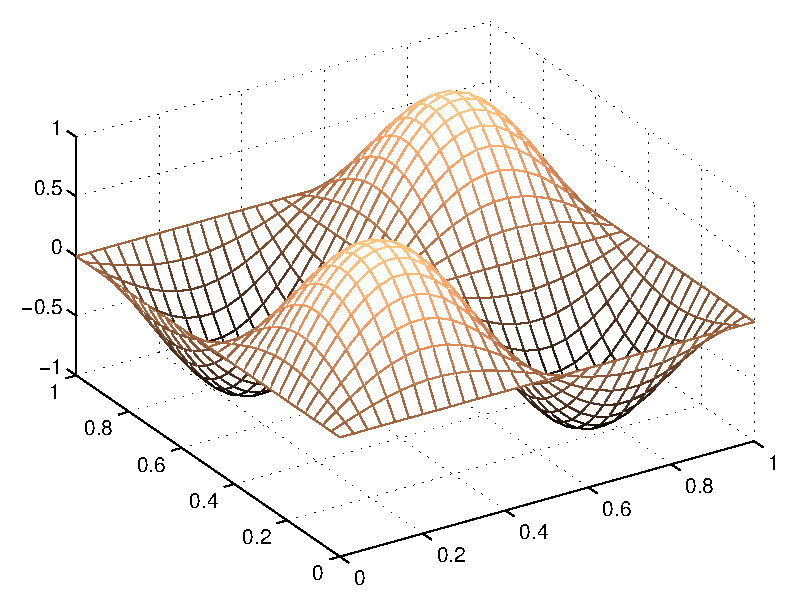
\includegraphics[width=0.4\textwidth]{../figs/sine_wave_funct3}}
	}
	\subfigure[tilting slope]{
		\centering
		{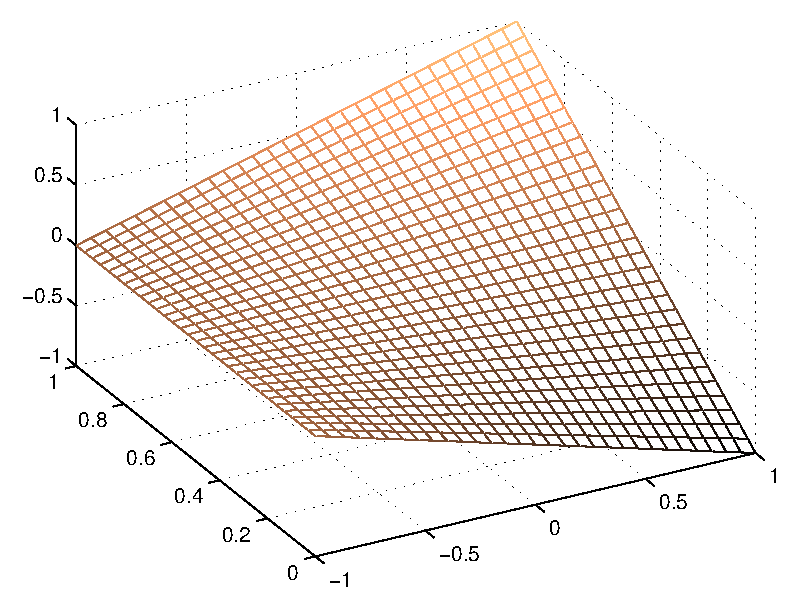
\includegraphics[width=0.4\textwidth]{../figs/tilting_slope_funct3}}
	}
\caption{Two additively unfaithful functions. Relevant variables are
  zeroed out under an additive approximation because every ``slice''
  of the function integrates to zero.}
\vskip-10pt
\end{figure*}


\begin{lemma}
\label{lem:general_int_reduction}
Let $F$ be a product distribution on $\mathbf{C}=[0,1]^s$ with density function $p$ which is positive on $\mathbf{C}$. Let
$X=(X_1,...,X_s) \sim F$. Let $f: \mathbf{C} \rightarrow \R$ be an
integrable function.
Let 
\begin{equation}
\begin{split}
f_k^*, \mu^* \coloneqq \argmin_{f_1,\ldots, f_s, \mu} \Bigl\{ \E \bigl( f(X) & -
 \sum_{k=1}^s f_k(X_k) -\mu \bigr)^2 \\
       & \,:\, \E f_k(X_k) = 0\Bigr\}.
\end{split}
\end{equation}
Then $\mu^* = \E f(X)$ and $f^*_k(x_k) = \E[ f(X) \given x_k] - \E f(X)$ and this solution is unique.
\end{lemma}

Lemma~\ref{lem:general_int_reduction} follows from the stationarity
conditions of the optimal solution. If $F$ is the uniform distribution,
then $f^*_k(x_k) = \int f(x_k, \mathbf{x}_{-k})
d\mathbf{x}_{-k}$.

\begin{example} We give two examples of additive unfaithfulness under
  the uniform distribution. First, consider the following function:
\[
\trm{(egg carton)} \quad f(x_1, x_2) = \sin( 2\pi x_1) \sin( 2 \pi x_2)
\]
defined for $(x_1, x_2) \in [0,1]^2$.  Then
$\int_{x_2} f(x_1, x_2) d x_2 = 0$ and
$\int_{x_1} f(x_1, x_2) d x_1 = 0$ for each $x_1$ and $x_2$. An additive approximation
would set $f_1 = 0$ and $f_2 = 0$.  Next, consider the function
\[
\trm{(tilting slope)} \quad f(x_1, x_2) = x_1 x_2
\]
defined for $x_1 \in [-1,1],\; x_2 \in [0,1]$.  In this case
$\int_{x_1} f(x_1, x_2) d x_1 = 0$ for each $x_2$; therefore, we expect $f_2 = 0$ under the additive approximation. This function, for every fixed $x_2$, is a zero-intercept linear function of $x_1$ with slope $x_2$.
\end{example}

In order to exploit additive models, it is important to understand when the
additive approximation accurately captures all of the relevant variables.
We call this property \emph{additive faithfulness}.

\begin{definition}
  Let $\mathbf{C}=[0,1]^s$, and $f:\mathbf{C}\rightarrow \R$. We say
  that $f$ \emph{depends on} coordinate $k$ if there exist $x'_k \neq
  x_k$ such that $f(x'_k, \mathbf{x}_{-k})$ and $f(x_k,
  \mathbf{x}_{-k})$ are different functions of $\mathbf{x}_{-k}$.

Let $F$ be a probability distribution on $\mathbf{C}$ and
assume without loss of generality that $\E f(X) = 0$. Let 
\begin{equation}
\begin{split}
f_k^*, \mu^* \coloneqq \argmin_{f_1,\ldots, f_s, \mu} \Bigl\{ 
             \E ( f(X) &- \sum_{k=1}^s f_k(X_k) -\mu )^2 \\
         &\,:\, \E f_k(X_k) = 0 \Bigr\}.
\end{split}
\end{equation}
We say that $f$ is \emph{additively faithful} under $F$ in case $f^*_k = 0$ iff $f$ does not depend on coordinate $k$. 
\end{definition}
% We can define the support $\trm{supp}(f) \coloneqq \{ k \,:\,
% \trm{$k$ is relevant to $f$}\}$. Let $f^* = \sum_{k=1}^s$, then $f$
% is additively faith if $\trm{supp}(f) = \trm{supp}(f^*)$.

Remarkably, under product distributions, a convex multivariate function can always be faithfully approximated by an additive function. 

\begin{theorem}
\label{thm:convex_faithful}
Let $F$ be a product distribution supported on $C=[0,1]^s$ with positive density $p$. If $f$ is convex and twice differentiable, then $f$ is additively faithful under $F$.
\end{theorem}

We give the full proof in Section~\ref{sec:faithful_proof} of the
Appendix, but pause here to provide some intuition. From
Lemma~\ref{lem:general_int_reduction}, we know that the
additive approximation zeroes out $k$ when, fixing $x_k$, every
``slice'' of $f$ integrates to zero. We prove
Theorem~\ref{thm:convex_faithful} by showing that ``slices'' of convex
functions that integrate to zero cannot be ``glued'' together while
still maintaining convexity.

Theorem~\ref{thm:convex_faithful} plays an important role in our
sparsistency analysis, where we show that the additive
approximation is variable selection consistent (or ``sparsistent''), even when the true function is not
additive.

\begin{remark}
  We assume twice differentiability in
  Theorem~\ref{thm:convex_faithful} to simplify the proof. We believe
  this smoothness condition is not necessary because every non-smooth
  convex function can be approximated arbitrarily well by a smooth
  one.  
\end{remark}
\begin{remark}
Without restrictions on the distribution, a convex
  function may not be additively faithful. Intuitively, an arbitrarily shaped
  density $p$
  may ``undo'' the convexity of $f$ so that the product
  $p(\mathbf{x}) \, f(\mathbf{x})$ resembles an egg carton or a
  tilting slope.  With appropriate conditions on the density $p$,
  however, it is possible to relax the independence assumption.  We leave this to
  future work.
\end{remark}

\section{Optimization for Sparse Convex Additive Models}

We now consider the following nonparametric regression problem
\begin{equation}\nonumber
          Y_{i} = f(\bds{x}_{i}) + \epsilon_{i} = 
                  \sum_{k=1}^{p}f_{k}(x_{ki}) + \epsilon_{i} \quad i=1,2,\cdots,n
\end{equation}
where $\bds{x}_{i}\in\mathbb{R}^{p}$ is the covariate, $Y_{i}$ is the
response and $\epsilon_{i}$ is mean zero noise. The regression function $f(\cdot)$ is the summation of 
functions $f_{k}(\cdot)$ in each variable dimension.  
We impose an additional constraint that each $f_{k}(\cdot)$ is 
an univariate convex function, which can be represented by its supporting hyperplanes, i.e.,
\begin{equation}\label{hyper}
      h_{kj} \geq h_{ki} + \beta_{ki}(x_{kj}-x_{ki}) \quad (\forall i,j)
\end{equation}
where $h_{ki}\coloneqq f_{k}(x_{ki})$ and $\beta_{ki}$ is the
subgradient at point $x_{ki}$. We apparently need $O(n^2 p)$ constraints to
impose the supporting hyperplane constraints, which is computationally
expensive for large scale problems.  In fact, only $O(np)$
constraints suffice, since univariate convex functions are
characterized by the condition that the subgradient, which is a scalar, must
increase monotonically. This observation leads to our optimization
program:
\begin{equation}\begin{split}\label{np}
       &\min_{\bds{h},\bds{\beta},\mu} \ \frac{1}{2n}\sum_{i=1}^{n}
                     \Bigl( Y_{i}-\sum_{k=1}^{p}h_{ki} - \mu \Bigr)^{2} 
                         + \lambda\sum_{k=1}^{p}\|\bds{\beta}_{k\cdot}\|_{\infty} \\
       &\ \textrm{s.t.} \ \sum_{i=1}^{n}h_{ki}=0,\; h_{k(i+1)} = h_{k(i)} + \beta_{k(i)}(x_{k(i+1)}-x_{k(i)}), 
                                 \ \beta_{k(i+1)} \geq \beta_{k(i)} \ (\forall k, i)
\end{split}\end{equation}
We introduce a mean parameter $\mu \in \R$ because $f$ may not have zero-mean. We can in fact solve $\mu$ explicitly here: the optimal $\mu = \frac{1}{n} \sum_{i=1}^n Y_i = \bar{Y}$ because of KKT and the constraints that $\sum_i h_{ki} = 0$.
$\{(1),(2),\ldots,(n)\}$ is a reordering of $\{1,2,\ldots,n\}$ such that $x_{k(1)}\leq{}x_{k(2)}\leq\cdots\leq{}x_{k(n)}$.  It is easy to verify that the constraints in (\ref{np}) satisfy the supporting hyperplane constraints, as
\begin{align*}
  \forall j\geq{}i, &h_{k(j)}-h_{k(i)}  = 
            \sum\limits_{t=i}^{j-1}(h_{k(t+1)}-h_{k(t)}) = 
            \sum\limits_{t=i}^{j-1}\beta_{k(t)}(x_{k(t+1)}-x_{k(t)})\\ 
      & \geq \beta_{k(i)}\sum\limits_{t=i}^{j-1}(x_{k(t+1)}-x_{k(t)}) = \beta_{k(i)}(x_{k(j)}-x_{k(i)}) \\
  \forall j<i, &h_{k(j)}-h_{k(i)} =
                \sum\limits_{t=j}^{i-1}(h_{k(t)}-h_{k(t+1)}) = 
                \sum\limits_{t=j}^{i-1}\beta_{k(t)}(x_{k(t)}-x_{k(t+1)}) \\ 
     & \geq \beta_{k(i)}\sum\limits_{t=j}^{i-1}(x_{k(t)}-x_{k(t+1)}) = \beta_{k(i)}(x_{k(j)}-x_{k(i)}), 
\end{align*}
The $\ell_\infty/\ell_1$ penalty
$\sum_{k=1}^{p}\|\bds{\beta}_{k\cdot}\|_{\infty}$ encourages group
sparsity of the vectors $\bds{\beta}_{k\cdot}$, and thus performs
variable selection.  We refer to this framework as the sparse convex
additive model (SCAM). Notice that if we replace $\beta_{k(i+1)} \geq
\beta_{k(i)}$ with $\beta_{k(i+1)}=\beta_{k(i)}$, the optimization
reduces to the lasso.  Note while one can use
supporting hyperplanes to the epigraph as in \eqref{eq:outer}, 
SCAM uses the \emph{inner  piece-wise linear function}
that approximates the graph with secant lines.


%\begin{SCfigure}
%\label{fig:outer_approximation}
%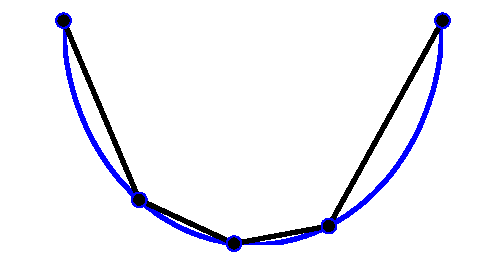
\includegraphics[width=0.3\textwidth]{figs/outer_approximation.pdf}
%\caption{With the 5 sample points $(X_i, h(X_i))$, the
%  black and the blue convex function represent equivalent fits. SCAM
%  chooses the inner piece-wise linear convex functions.}
%\end{SCfigure}

The SCAM optimization in (\ref{np}) is a quadratic program (QP) with $O(np)$ variables and $O(np)$ constraints. The optimal $\mu$ has a closed form solution of $\mu = \frac{1}{n}\sum_{i=1}^n Y_i$, which is easy to derive from the KKT theorem and the constraints that $\sum_i h_{ki} = 0$ for all $k$.
Directly applying a QP solver for $\bds{h}, \bds{\beta}$ would be computationally expensive for relatively large $n$ and $p$. However, notice that variables
in different feature dimensions are only coupled in the term $(Y_{i}-\sum_{k=1}^{p}h_{ki})^{2}$. Hence, we can apply the block coordinate descent method,
where in each step we solve the following QP subproblem for
$\{\bds{h}_{k\cdot},\bds{\beta}_{k\cdot}\}$ with the other variables fixed:
\begin{equation}\begin{split}\nonumber
       &\min_{\bds{h}_{k\cdot},\bds{\beta}_{k\cdot},\gamma_{k}} 
             \ \frac{1}{2n}\sum_{i=1}^{n}\Bigl((Y_{i}-\bar{Y}-\sum_{r\neq{k}}h_{ri})-h_{ki}\Bigr)^{2} 
                      + \lambda\gamma_{k} \\
        &\ \textrm{s.t.} \ \sum_{i=1}^{n}h_{ki}=0, \ h_{k(i+1)} = h_{k(i)} + \beta_{k(i)}(x_{k(i+1)}-x_{k(i)}), \ \beta_{k(i+1)} \geq \beta_{k(i)}, \ -\gamma_{k}\leq\beta_{k(i)}\leq\gamma_{k} \ (\forall i).
\end{split}\end{equation}
The extra variable $\gamma_{k}$ is introduced to deal with the $\ell_{\infty}$ norm. This QP subproblem involves $O(n)$ variables, $O(n)$ constraints and a sparse structure, 
which can be solved efficiently using optimization packages (e.g., MOSEK: \verb+http://www.mosek.com/+).  We cycle through all feature dimensions ($k$) from $1$ to $p$ multiple times until convergence.
Empirically, we observe that the algorithm converges in only a few cycles. We also implemented an ADMM solver for (\ref{np}), but found that it is not as efficient as this QP solver.

After optimization, the function estimator for any input data $\bds{x}_j$ is, according to (\ref{hyper}),
\begin{equation}\nonumber
      f(\bds{x}_j) = \sum_{k=1}^{p}f_k(x_{kj})+\mu = \sum_{k=1}^{p}\max_{i} \{h_{ki}+\beta_{ki}(x_{kj}-x_{ki})\} + \mu.
\end{equation} 


\subsection{Alternative Formulation}
Optimization (\ref{np}) can be reformulated in terms of the 2nd derivatives. The alternative formulation replaces the ordering
constraints $\beta_{k(i+1)} \geq \beta_{k(i)}$ with positivity
constraints, which simplifies theoretical analysis.
Define $d_{k(i)}$ as the second derivative:
$d_{k(1)} = \beta_{k(1)}$, and $d_{k(2)} =
\beta_{k(2)} - \beta_{k(1)}$. The convexity constraint is
equivalent to the constraint that $d_{k(i)} \geq 0$ for all $i >
1$.

It is easy to verify that $\beta_{k(i)} = \sum_{j \leq i} d_{k(i)}$ and 
\[
f_k(x_{k(i)}) = f_k({x_{k(1)}}) +d_{k(1)} ( x_{k(i)}
- x_{k(1)}) + d_{k(2)} ( x_{k(i)} - x_{k(2)}) + \cdots + d_{k(i-1)} ( x_{k(i)} - x_{k(i-1)})
\]
We can write this more compactly in matrix notations. First define $\Delta_{k(j)}(x_{ki}) = \max( x_{ki} - x_{k(j)}, 0)$. 
\[
\left[ \begin{array}{c}
    f_k(x_{k1}) \\
    ... \\
    f_k(x_{kn}) \\
\end{array} \right] =
\left[ \begin{array}{ccc}
    \Delta_{k(1)}(x_{k1}) & ... & \Delta_{k(n-1)}(x_{k1}) \\
    ... & & \\
    \Delta_{k(1)}(x_{kn}) & ... & \Delta_{k(n-1)}(x_{kn}) 
\end{array} \right]
\left[ \begin{array}{c}
    d_{k(1)} \\
    ... \\
    d_{k(n-1)}
\end{array} \right] \coloneqq \Delta_k d_k
\]
Where $\Delta_k$ is a $n\times n-1$ matrix such that $\Delta_k(i,j) = \Delta_{k(j)}(x_{k(i)})$ and $d_k = (d_{k(1)} ,..., d_{k(n-1)})$. We can now reformulate (\ref{np}) as an equivalent optimization program with only centering and positivity constraints:
\begin{align}
\min_{d_k \in \R^{n-1}, c_k \in \R,\mu \in \R}& \frac{1}{2n} 
       \Bigl\| Y - \bar{Y}\mathbf{1}_n - \sum_{k=1}^p ( \Delta_k d_k - c_k \mathbf{1}_n) \Bigr\|_2^2 
               + \lambda_n \sum_{k=1}^p \|d_k\|_1  & \label{opt:alternate_opt} \\
\trm{s.t. $\forall k$, }  & d_{k(2)}, \ldots , d_{k(n-1)} \geq 0 	
               \qquad &\trm{(convexity)} \nonumber \\ 
	& c_k = \frac{1}{n} \mathbf{1}_n^\tran \Delta_k d_k 	
               \qquad &\trm{(centering)} \nonumber 
\end{align}
$\|d_k\|_1$ is not identical to $\|\bds{\beta}_{k\cdot}\|_{\infty}$, but it is easy to verify that $\|\bds{\beta}_{k\cdot}\|_{\infty} \leq \|d_k\|_1 \leq 2\|\bds{\beta}_{k\cdot}\|_{\infty}$.

\begin{remark}
\label{rem:bounded_lipschitz_constraints}
For parts of our theoretical analysis, we will also impose onto (\ref{opt:alternate_opt}) a boundedness constraint $-B \mathbf{1}_n \leq \Delta_k d_k + c_k \mathbf{1}_n \leq B \mathbf{1}_n$ which constrains that $\|f_k \|_\infty \leq B$, or a Lipschitz constraint $\|d_k\|_1 \leq L$ which constrains that $f_k$ must be $L$-Lipschitz. We use these constraints only in the proof for technical reasons; we never need nor use these constraints in our experiments.
\end{remark}



\section{Analysis of Variable Selection Consistency}

We divide our analysis into two parts. We first establish a sufficient
\emph{deterministic} condition for sparsistency.  We then consider the
stochastic setting and argue that the deterministic conditions hold with high probability. 

\subsection{Deterministic Setting}

We follow \cite{Wain:09a} and define the \emph{restricted regression} purely for theoretical purposes.
\begin{definition}
In \emph{restricted regression}, we restrict the indices $k$ in
optimization (\ref{opt:alternate_opt}) to lie in the support $S$ instead of ranging from $1,...,p$. 
\end{definition}

Our analysis then differs from the now-standard ``primal-dual witness
technique''~\cite{Wain:09a}. Primal-dual witness explicitly solves all the dual variables, but because our optimization is more complex, we do not solve the dual variables on $S$; we instead write the dual variables on $S^c$ as a function of the restricted regression \emph{residual}, which is implicitly a function of the dual variables on $S$.

\begin{theorem} (Deterministic setting)
\label{thm:deterministic}
Let $\{\hat{d}_k, \hat{c}_k\}_{k \in S}$ be the minimizer of the restricted regression, that is, the solution to optimization (\ref{opt:alternate_opt}) where we restrict $k \in S$. Let $\hat{d}_k = 0$ and $ \hat{c}_k = 0$ for $k \in S^c$.
Let $\hat{r} \coloneqq Y - \bar{Y}\mathbf{1}_n - \sum_{k \in S} (\Delta_k \hat{d}_k -
\hat{c}_k \mathbf{1}_n)$ be the restricted regression residual. For $k
\in \{1,...,p\}$, Let $\Delta_{k, j} \in R^n$ be the $j$-th column of $\Delta_k$, i.e. $\max( X_k - X_{k (j)} \mathbf{1}_n, 0)$. \\

Suppose for all $j$ and all $k\in S^c$, $\lambda_n > | \frac{1}{n}
\hat{r}^\tran \Delta_{k,j}|$. Then $\hat{\mu}$ and $\hat{d}_k, \hat{c}_k$ for $k=1,...,p$ is an optimal solution to the full regression \ref{opt:alternate_opt}. Furthermore, any solution to the optimization program \ref{opt:alternate_opt} must be zero on $S^c$.
\end{theorem}

This result holds regardless of whether we impose the boundedness and Lipschitz conditions in optimization~\ref{opt:alternate_opt}.
The full proof of Theorem~\ref{thm:deterministic} is in Section~\ref{sec:deterministic_proof} of the Appendix.

\begin{remark}
  The incoherence condition of \cite{Wain:09a} is implicitly encoded
  in our condition on $\lambda_n, \hat{r}, \Delta_{k,j}$. We can
  reconstruct the incoherence condition if we assume that the true
  function $f_0$ is linear and that our fitted functions $\hat{f}_k$
  are linear as well.
\end{remark}

Theorem~\ref{thm:deterministic} allows us to analyze false negative
rates and false positive rates separately. To control false positives,
we study when the condition $\lambda_n > | \frac{1}{n} \hat{r}^\tran
\Delta_{k,j}|$ is fulfilled for all $j$ and all $k \in S^c$. To
control false negatives, we study the restricted regression.

\subsection{Probabilistic Setting}

We use the following statistical setting:

\begin{packed_enum}
\item Let $F$ be a distribution supported and positive on $\mathcal{X}=[-b,b]^p$. Let $X^{(1)},..., X^{(n)} \sim F$ be iid.
\item Let $Y = f_0(X) + \epsilon$ where $\epsilon$ is zero-mean noise. Let $Y^{(1)},...,Y^{(n)}$ be iid.
\item Let $S = \{1,...,s\}$ denote the relevant variables where $s\leq p$, i.e.,
  $f_0(X) = f_0(X_S)$.
\item Let $f^*_1,...,f^*_s \coloneqq \argmin_{f_1,...,f_s} \{ \E(f_0(X) - \sum_{k=1}^s f_k(X_k))^2 \,|\, \E[f_k(X_k)] = 0 \}$.
\end{packed_enum}

Each of our theorems will use a subset of the following assumptions:
\begin{packed_enum}
\item[A1:] $X_S, X_{S^c}$ are independent.  \ A1': $\{ X_k \}_{k \in S}$ are independent.
\item[A2:] $\|f_0\|_\infty \leq sB$ \  A2': $f_0$ is convex,
  twice-differentiable, $L$-Lipschitz, and $\trm{supp}(f_0) = S$.
\item[A3:] Suppose $\epsilon$ is mean-zero sub-Gaussian, independent of $X$, with sub-Gaussian scale $\sigma$, i.e. for all $t \in \R$, $\E e^{t \epsilon} \leq \E e^{\sigma^2 t^2 / 2}$.
\item[A4:] For all $k=1,...,s$, $\E(f^*_s(X_k))^2 \geq \alpha$ for some positive constant $\alpha$.
\end{packed_enum}

We will use assumptions A1, A2, A3 to control the probability of false
positives and the stronger assumptions A1', A2', A3, A4 to control the
probability of false negatives.  Assumption A4 can be
weakened so that the relevant functions satisfy
$\E(f^*_s(X_k))^2 \geq \alpha_n$ for $\alpha_n$ decaying to zero 
at an appropriate rate.



\begin{remark}
  We make strong assumptions on the covariates in A1 in order to make
  very weak assumptions on the true regression function $f_0$ in
  A2. In particular, we do not assume that $f_0$ is additive. Relaxing
  these assumptions is an interesting direction for future work. 
  %Strong assumptions on the covariates are not uncommon in nonparametric
  %variable selection analysis~\cite{lafferty2008rodeo}. 
  %[TODO: refer to correlated design experiment].
\end{remark}

\begin{remark}
Assumption A4 ensures that the relevant variables are ``relevant enough''. Under A4, the population risk of an additive function with $s-1$ components is at least $\alpha$ larger than the population risk of the optimal additive function with $s$ components. Lemma~\ref{lem:minus_one_risk_increase} in section~\ref{sec:false_negative_proof} of the appendix.
\end{remark}

\begin{theorem} (Controlling false positives) 
\label{thm:false_positive}
Suppose assumptions A1, A2, A3 hold. Suppose also that we run optimization~\eqref{opt:alternate_opt} with the $B$-boundness constraint. Let $c,C$ be absolute constants.
Suppose $\lambda_n \geq c b (sB + \sigma) \sqrt{ \frac{s}{n} \log n
  \log (pn)}$.  Then with probability at least $ 1 - \frac{C}{n}$, for all $j,k$, $\lambda_n >  | \frac{1}{n} \hat{r}^\tran \Delta_{k,j}|$.
Therefore, any solution to the full regression (\ref{opt:alternate_opt}), with boundedness constraint, is zero on $S^c$. 
\end{theorem}

The proof of Theorem~\ref{thm:false_positive} exploits independence of
$\hat{r}$ and $\Delta_{k,j}$ from A1, and then uses concentration of
measure results to argue that $| \frac{1}{n} \hat{r}^\tran
\Delta_{k,j}|$ concentrates around zero at a desired rate. The fact
that $\hat{r}$ is a centered vector is crucial to our proof, and our
theory thus further illustrates the importance of imposing the
centering constraints in optimization \eqref{opt:alternate_opt}. Our
proof uses the concentration of the average of
data sampled \emph{without} replacement
\cite{serfling1974probability}, illustrating that the proof method is not a
trivial application of existing techniques. The full proof of
Theorem~\ref{thm:false_positive} is in
Section~\ref{sec:false_positive_proof} of the Appendix.

\begin{theorem} (Controlling false negatives)
\label{thm:false_negative}
Suppose assumptions A1', A2', A3, A4 hold. Let $\ds \hat{f} = \{ \hat{d}_k, \hat{c}_k\}_{k\in S}$ be any solution to the restricted regression with both the $B$-boundedness and $L$-Lipschitz constraint. Let $c,C$ be absolute constants.
Suppose $s L \lambda_n \rightarrow 0$ and $bL (B+\sigma)B\sigma \sqrt{\frac{s^5}{n^{4/5}} \log sn} \rightarrow 0$.
Then, for sufficiently large $n$, $\hat{f}_k = (\hat{d}_k, \hat{c}_k)
\neq 0$ for all $k \in S$ with probability at least $1-\frac{C}{n}$.
\end{theorem}

This is a finite sample version of
Theorem~\ref{thm:convex_faithful}. We need stronger assumptions in
Theorem~\ref{thm:false_negative} to use our additive faithfulness
result, Theorem~\ref{thm:convex_faithful}. We also include an extra
Lipschitz constraint so that we can use existing covering number
results \cite{Bronshtein:76}. Recent work
\cite{Guntu:13} shows that the Lipschitz constraint
is not required with more advanced empirical process theory
techniques. We give the full proof of Theorem~\ref{thm:false_negative}
in Section~\ref{sec:false_negative_proof} of the Appendix.

Combining Theorem~\ref{thm:false_positive} and
~\ref{thm:false_negative} and ignoring dependencies on $b,B,L,\sigma$,
we have the following result.
\begin{corollary}
  Assume A1', A2', A3, A4. Let $\lambda_n = \Theta\left( \sqrt{
  \frac{s^3}{n} \log n \log (pn)} \right)$. Suppose $s \lambda_n
  \rightarrow 0$ and $\sqrt{\frac{s^5}{n^{4/5}} \log sn} \rightarrow
  0$. Let $\hat{f_n}$ be a solution to (\ref{opt:alternate_opt}) with
  boundedness and Lipschitz constraints. Then 
  $\P( \trm{supp}(\hat{f_n}) = \trm{supp}(f_0) ) \rightarrow 1$.
\end{corollary}
The above corollary implies that sparsistency is achievable at the same exponential scaling of the ambient dimension $p = O(\exp(n^c)), c<1$ rate as parametric models. The cost of nonparametric modeling is reflected in the scaling with respect to $s$, which can only scale at $o(n^{4/25})$.

%\textbf{Comparison with Related Work.} 


% DO NOT CHANGE; RefTex variables -minx
 
%%% Local Variables: ***
%%% mode:latex ***
%%% TeX-master: "scam_icml.tex" ***
%%% End: ***

\section{Experiments}
%\subsection{Simulations}
We first illustrate our methods using a simulation of the following regression problem
\begin{equation}\nonumber
         y_i = \bds{x}_{iS}^{\top}\bds{Q}\bds{x}_{iS} + \epsilon_i \quad (i=1,2,\ldots,n).
\end{equation}
Here $\bds{x}_{i}$ denotes data sample $i$ drawn from $\mathcal{N}(\bds{0},\bds{I}_{p})$, 
$\bds{x}_{iS}$ is a subset of $\bds{x}_i$ with dimension $|S|=5$, where $S$ represents the active feature set, and 
$\epsilon_i$ is the additive noise drawn from $\mathcal{N}(0,1)$. 
$\bds{Q}$ is a symmetric positive definite matrix of dimension $|S|\times{}|S|$. 
Notice that if $\bds{Q}$ is diagonal, then the true function is convex additive; otherwise the true function is convex but not additive.
For all the simulations in this section, we set $\lambda=4\sqrt{{\log(np)}/{n}}$.

In the first simulation, we set $\bds{Q}=\bds{I}_{|S|}$ (the additive
case), and choose $n=100, 200,\ldots,1000$ and $p=64,128,256,512$.
For each $(n,p)$ combination, we generate $200$ independent data
sets. For each data set we use SCAM to infer the model parameterized
by $\bds{h}$ and $\bds{\beta}$; see equation \eqref{np}. If
$\|\bds{\beta}_{k\cdot}\|_{\infty}<10^{-8}\ (\forall k\not\in{}S)$ and
$\|\bds{\beta}_{k\cdot}\|_{\infty}>10^{-8}\ (\forall k\in{}S)$, then
we declare correct support recovery. We then plot the probability of
support recovery over the $200$ data sets in Figure \ref{Support}(a).  We
observe that SCAM performs consistent variable selection when the true
function is convex additive.  
To give the reader a
sense of the running speed, the code runs in about $2$ minutes on one
data set with $n=1000$ and $p=512$, on a MacBook with 2.3 GHz Intel
Core i5 CPU and 4 GB memory.

In the second simulation, we study the case in which the true function
is convex but not additive. We generate four $\bds{Q}$ matrices
plotted in Figure \ref{Support}(b), where the diagonal elements are all $1$ and
the off-diagonal elements are $0.5$ with probability $\alpha$
($\alpha=0,0.2,0.5,1$ for the four cases). We fix $p=128$ and choose
$n=100,200,\ldots,1000$. We again run the SCAM optimization on $200$
independently generated data sets and plot the probability of recovery
in Figure \ref{Support}(c). The results demonstrate that SCAM performs
consistent variable selection even if the true function is not additive (but
still convex).

In the third simulation, we study the case of correlated design, where
$\bds{x}_{i}$ is drawn from $\mathcal{N}(\bds{0},\bds{\Sigma})$
instead of $\mathcal{N}(\bds{0},\bds{I}_{p})$, with
$\Sigma_{ij}=\nu^{|i-j|}$. We use the non-additive $\bds{Q}$ with
$\alpha=0.5$ and fix $p=128$.  The recovery curves for $\nu=02, 0.4,
0.6, 0.8$ are depicted in Figure \ref{Support}(d). As can be seen, for
design of moderate correlation, SCAM can still select relevant
variables well.


%\begin{figure}[!htpb]
%        \centering
%        \begin{subfigure}[b]{0.45\textwidth}
%                \centering
%                \includegraphics[width=\textwidth]{figs/Curve1}
%                 \caption{Additive model.}
%                \label{Curve1}
%        \end{subfigure}
%        \begin{subfigure}[b]{0.45\textwidth}
%                \centering
%                \includegraphics[width=\textwidth]{figs/Q}
%                \caption{Four $\bds{Q}$ matrices.}
%                \label{Q}
%        \end{subfigure}\\
%        \begin{subfigure}[b]{0.45\textwidth}
%                \centering
%                \includegraphics[width=\textwidth]{figs/Curve2}
%                \caption{Additive and non-additive models.}
%                \label{Curve2}
%        \end{subfigure}
%        \begin{subfigure}[b]{0.45\textwidth}
%                \centering
%                \includegraphics[width=\textwidth]{figs/Curve3}
%                \caption{Correlated design for non-additive model.}
%                \label{Curve3}
%        \end{subfigure}
%        \caption{Result of support recovery.}\label{Support}
%\end{figure}

%\begin{figure}[ht]
%\begin{center}
%\begin{tabular}{cccc}
%\hskip-20pt
%\includegraphics[width=.27\textwidth]{figs/Curve1} &
%\hskip-17pt
%\includegraphics[width=.27\textwidth]{figs/Q} &
%\hskip-17pt
%\includegraphics[width=.27\textwidth]{figs/Curve2} &
%\hskip-17pt
%\includegraphics[width=.27\textwidth]{figs/Curve3}  \\
%(a) additive model & (b) four $\bds{Q}$ matrices &
%(c) non-additive models & (d) correlated design
%\end{tabular}
%\end{center}
%\caption{Result of support recovery.}\label{Support}
%\end{figure}


%\subsection{Boston housing data}

We next use the Boston housing data rather than simulated data. This data set
contains 13 covariates, 506 samples and one response variable
indicating housing values in suburbs of Boston. The data and detailed description
can be found on the UCI Machine Learning Repository website~\verb+http://archive.ics.uci.edu/ml/datasets/Housing+. 

We first use all $n=506$ samples (with normalization) to train SCAM, using
a set of candidate $\{\lambda^{(t)}\}$ with $\lambda^{(1)}=0$ (no regularization). For each $\lambda^{(t)}$
we obtain a subgradient matrix $\bds{\beta}^{(t)}$ with $p=13$ rows. The non-zero
rows in this matrix indicate the variables selected using $\lambda^{(t)}$. 
We plot $\|\bds{\beta}^{(t)}\|_{\infty}$ and the row-wise mean of $\bds{\beta}^{(t)}$ versus the normalized
norm $\frac{\|\bds{\beta}^{(t)}\|_{\infty,1}}{\|\bds{\beta}^{(1)}\|_{\infty,1}}$ in Figures \ref{Boston}(a) and \ref{Boston}(b).
As a comparison we plot the LASSO/LARS result in a similar way in Figure \ref{Boston}(c).
From the figures we observe that the first three variables selected by SCAM
and LASSO are the same: LSTAT, RM and PTRATIO, which is consistent with previous findings~\cite{SpAM:07}.
The fourth variable selected by SCAM is TAX (with $\lambda^{(t)}=0.09$).
We then refit SCAM with only these four variables without regularization, and plot the inferred additive
functions in Figure \ref{Boston}(e). As can be seen, these functions contain clear nonlinear effects which cannot be captured
by LASSO. The shapes of these functions are in agreement with those obtained by SpAM~\cite{SpAM:07}.

Next, in order to quantitatively study the predictive performance, we run 10 times 5-fold cross validation, following
the same procedure described above (training, variable selection and
refitting).  A plot of the mean and standard
deviation of the predictive Mean Squared Error (MSE) in in Figure \ref{Boston}(d). Since for SCAM the same $\lambda^{(t)}$ may lead to
slightly different number of selected features in different folds and runs, the values on the x-axis (average number of selected features)
for SCAM are not necessarily integers. Nevertheless, the figure clearly shows that SCAM has a much lower predictive MSE than LASSO. 
We also compared the performance of SCAM with that of Additive Forward Regression (AFR) presented in~\cite{Xi:09}, and found that they are similar.
The main advantages of SCAM compared with AFR and SpAM are 1) there are no other tuning parameters (such as bandwidth)
besides $\lambda$; 2) SCAM is formulated as a convex program, which guarantees a global optimum.

%\begin{figure}[!htpb]
%        \centering
%        \begin{subfigure}[b]{0.45\textwidth}
%                \centering
%                \includegraphics[width=\textwidth]{figs/Additive}
%                 \caption{Variable selection result using SCAM.}
%                \label{SCAM}
%        \end{subfigure}
%        \begin{subfigure}[b]{0.45\textwidth}
%                \centering
%                \includegraphics[width=\textwidth]{figs/Additive1}
%                 \caption{Variable selection result using SCAM.}
%                \label{SCAM1}
%        \end{subfigure}\\
%        \begin{subfigure}[b]{0.45\textwidth}
%                \centering
%                \includegraphics[width=\textwidth]{figs/LASSO}
%                \caption{Variable selection result using LASSO.}
%                \label{LASSO}
%        \end{subfigure}
%        \begin{subfigure}[b]{0.45\textwidth}
%                \centering
%                \includegraphics[width=\textwidth]{figs/MSE}
%                 \caption{Predictive MSE of SCAM and LASSO.}
%                 \label{MSE}
%        \end{subfigure}\\
%        \begin{subfigure}[b]{0.45\textwidth}
%                \centering
%                \includegraphics[width=\textwidth]{figs/Convex}
%                \caption{Inferred additive convex functions by SCAM.}
%                \label{Convex}
%        \end{subfigure}
%        \caption{Results on Boston housing data.}\label{Boston}
%\end{figure}


\begin{figure*}[!t]
\begin{center}
\begin{tabular}{cccc}
\hskip-20pt
\includegraphics[width=.29\textwidth]{../figs/Curve1} &
\hskip-20pt
\includegraphics[width=.29\textwidth]{../figs/Q} &
\hskip-20pt
\includegraphics[width=.29\textwidth]{../figs/Curve2} &
\hskip-20pt
\includegraphics[width=.29\textwidth]{../figs/Curve3}  \\
\hskip-10pt (a) additive model & 
\hskip-10pt (b) four $\bds{Q}$ matrices &
\hskip-10pt (c) non-additive models & 
\hskip-10pt (d) correlated design
\end{tabular}
\end{center}
\caption{Support recovery results where the additive assumption is
  correct (a), incorrect (b), (c), and with correlated design (d).}\label{Support}
\vskip10pt

\begin{center}
\begin{tabular}{ccc}
\hskip-10pt
  \includegraphics[width=.35\textwidth]{../figs/Additive} &
\hskip-25pt
  \includegraphics[width=.35\textwidth]{../figs/Additive1} &
\hskip-25pt
  \includegraphics[width=.35\textwidth]{../figs/LASSO} 
\\
\hskip-10pt 
SCAM $\|\beta_k\|_\infty$ paths & 
\hskip-25pt 
SCAM $\text{mean}(\beta_k)$ paths &
\hskip-25pt
LASSO $\beta_k$ paths
\end{tabular}
\begin{tabular}{cc}
  \includegraphics[width=.37\textwidth]{../figs/MSE} &
  \includegraphics[width=.43\textwidth]{../figs/Convex}
\\
predictive MSE & inferred functions from SCAM
\end{tabular}
\end{center}
\caption{Results on Boston housing data, showing regularization paths,
 MSE and fitted functions.}\label{Boston}
\end{figure*}

\section{Discussion}

We have introduced a framework for estimating high dimensional but
sparse convex functions.  Because of the special properties of
convexity, variable selection for convex functions enjoys additive
faithfulness---it suffices to carry out variable selection over an
additive model, in spite of the approximation error this introduces.
Sparse convex additive models can be optimized using block coordinate
quadratic programming, which we have found to be effective and
scalable.  We established variable selection consistency results,
allowing exponential scaling in the ambient dimension.  We expect
that the technical assumptions we have used in these analyses can be
weakened; this is one direction for future work.  Another interesting
direction for building on this work is to allow for additive models that
are a combination of convex and concave components.  If the
convexity/concavity of each component function is known, this again
yields a convex program.  The challenge is to develop a method to
automatically detect the concavity or convexity pattern of the
variables.





\bibliography{local}
\bibliographystyle{icml2014}

\newpage
\onecolumn{
\section{Appendix}
 
 
 \subsection{Proof of the Deterministic Condition for Sparsistency}
 \label{sec:deterministic_proof}
 
We restate Theorem~\ref{thm:deterministic} first for convenience. 
 
\begin{theorem} 
The following holds regardless of whether we impose the Lipschitz condition in optimization~\ref{opt:alternate_opt} and optimization~\ref{opt:alternate_opt_concave}.

Let $\{\hat{d}_k \}_{k \in S}$ be a minimizer of the restricted regression, that is, the solution to optimization (\ref{opt:alternate_opt}) where we restrict $k \in S$. 
Let $\hat{r} \coloneqq Y - \sum_{k \in S} \bar{\Delta}_k \hat{d}_k$ be the restricted regression residual. \\

Suppose for all $k\in S^c$, for all $i=1,...,n$, $\lambda_n > | \frac{1}{2n}
\hat{r}^\tran \mathbf{1}_{(i:n)}|$ where $\mathbf{1}_{(i:n)}$ is 1 on the coordinates of the $i$-th largest to the $n$-th largest entries of $X_k$ and 0 elsewhere.\\

Then the following are true:
\begin{enumerate}
\item Let $\hat{d}_k = 0$ for $k \in S^c$, then \{$\hat{d}_k\}_{k=1,...,p}$ is an optimal solution to optimization~\ref{opt:alternate_opt}. Furthermore, any solution to the optimization program \ref{opt:alternate_opt} must be zero on $S^c$.
\item For all $k \in S^c$, the solution to optimization~\ref{opt:alternate_opt_concave} must be 0 and must be unique.
\end{enumerate}
\end{theorem}


\begin{proof} 
We will omit the Lipschitz constraint in our proof here. It is easy to add that in and check that the result of the theorem still holds.\\

We first consider the first item in the conclusion of the theorem.

We will show that with $\{\hat{d}_k\}_{k=1,..,p}$ as constructed, we can set the dual variables to satisfy complementary slackness and stationary conditions: $\nabla_{d_k} \mathcal{L}(\hat{d})  = 0$ for all $k$.\\ 

The Lagrangian is
\begin{equation}
\label{eqn:full_lagrange}
\mathcal{L}( \{ d_k \}, \nu) = 
  \frac{1}{2n} \Big\| 
    Y - \sum_{k=1}^p  \bar{\Delta}_k d_k  \Big\|_2^2 + 
    \lambda \sum_{k=1}^p \| \bar{\Delta}_k d_k \|_\infty -
    \sum_{k=1}^p \sum_{i=2}^{n-1} \nu_{ki} d_{ki} 
\end{equation}
with the constraint that $\nu_{ki} \geq 0$ for all $k,i$.

Because $\{\hat{d}_k\}_{k \in S}$ is by definition the optimal solution of the restricted regression, it is a consequence that stationarity holds for $k \in S$, that is, $\partial_{ \{ d_k \}_{k \in S} } \mathcal{L}(d) = 0$, and that the dual variables $\nu_k$ for $k \in S$ satisfy complementary slackness.

We now verify that stationarity holds also for $k \in S^c$. We fix one dimension $k \in S^c$ and let $\hat{r} = Y - \sum_{k' \in S} \bar{\Delta}_{k'} \hat{d}_{k'}$. 

The Lagrangian form of the optimization, in term of just $d_k$, is
\[
\mathcal{L}(d_k, \nu_k) =
  \frac{1}{2n} \big\| Y - \sum_{k' \in S} \bar{\Delta}_{k'} d_{k'} 
  -  \bar{\Delta}_k d_k \big\|_2^2 
   + \lambda \| \bar{\Delta}_k d_k\|_\infty
  - \sum_{i=2}^{n-1} \nu_{ki} d_{ki}
\]
with the constraint that $v_i \geq 0$ for all $i$. 

The derivative of the Lagrangian is:
\begin{align*}
\partial_{d_k} \mathcal{L}(d_k) =  -\frac{1}{n} \bar{\Delta}_k^\tran ( Y - \sum_{k'\in S} \bar{\Delta}_{k'} d_{k'}  - \bar{\Delta}_k d_k )
        + \lambda \bar{\Delta}_k^\tran \mathbf{u}
      - \nu_k
\end{align*}
where $\mathbf{u}$ is the subgradient of $\| \bar{\Delta}_k d_k \|_\infty$, an $n$-vector such that $\| \mathbf{u}_T \|_1 = 1$ where $T = \{ i \,:\,  (\bar{\Delta}_k d_k)_i = \| \bar{\Delta}_k d_k \|_\infty \}$.

We now substitute in $d_{k'} = \hat{d}_{k'}$ for $k' \in S$, $d_k = 0$ for $k \in S$, and $r = \hat{r}$ and show that the duals can be set in a way to ensure that the derivatives are equal to 0.

\begin{align*}
\partial_{d_k} \mathcal{L}(\hat{d}_k) = -\frac{1}{n} \bar{\Delta}_k^\tran\hat{r} + \lambda \bar{\Delta}_k^\tran \mathbf{u}
           - \nu_k = 0 
\end{align*}
where $\| \mathbf{u} \| \leq 1$ and $\nu_k \geq 0$. It clear that to show stationarity, we only need to show that $-\frac{1}{n} \bar{\Delta}_k^\tran \hat{r} + \lambda \bar{\Delta}_k^\tran \mathbf{u} \geq 0$ hwere the inequality is element-wise.

Let us reorder the samples so that the $i$-th sample is the $i$-smallest sample. \\

We will construct $\gamma = 0$, and $\mathbf{u} = (-a, 0, ..., a)$ for some $0 < a < 1/2$. (coordinates of $\mathbf{u}$ correspond to the new sample ordering) We then just need to show that
\begin{align*}
- \frac{1}{n} \bar{\Delta}_k^\tran \hat{r} + \lambda \bar{\Delta}_k^\tran \mathbf{u} &\geq 0 \quad \Leftrightarrow \\
- \frac{1}{n} \Delta_k^\tran \hat{r} + \lambda \Delta_k^\tran \mathbf{u} &\geq 0 \quad \Leftrightarrow\\
- \frac{1}{n} \sum_{i > j} (X_{ki} - X_{kj}) \hat{r}_i + \lambda (X_{kn} - X_{kj})a &\geq 0 \quad 
   \textrm{for each } j \\
- \frac{1}{n} \sum_{i > j} \sum_{j < i' \leq i} \mathsf{gap}_{i'} \hat{r}_i 
    + \lambda (X_{kn} - X_{kj})a &\geq 0 \\
- \frac{1}{n} \sum_{i' > j} \mathsf{gap}_{i'} \sum_{i \geq i'} \hat{r}_i 
    + \lambda (X_{kn} - X_{kj})a &\geq 0 \\
- \frac{1}{n} \sum_{i' > j} \mathsf{gap}_{i'} \mathbf{1}_{(i':n)}^\tran \hat{r} 
   + \lambda (X_{kn} - X_{kj})a &\geq 0 
\end{align*}
where $\mathsf{gap}_i = X_{ki} - X_{k,i-1}$. If $\frac{1}{2n} |\mathbf{1}_{(i:n)}^\tran \hat{r}| \leq \lambda a$ for all $i=1,...,n$, then we have that:

\begin{align*}
- \frac{1}{n} \sum_{i' > j} \mathsf{gap}_{i'} \mathbf{1}_{i':n}^\tran \hat{r}
   + \lambda (X_{kn} - X_{kj})a &\geq 0 \quad \Leftrightarrow \\
- \sum_{i' > j} \mathsf{gap}_{i'} \lambda a + \lambda (X_{kn} - X_{kj}) a &\geq 0\\
- (X_{kn} - X_{kj}) \lambda a + \lambda (X_{kn} - X_{kj}) a &\geq 0
\end{align*}

We have thus proven that there exist one solution $\{ \hat{d}_k \}_{k=1,...,p}$ such that $\hat{d}_k = 0$ for all $k \in S^c$. Furthermore, we have shown that the subgradient variables $\mathbf{u}_k$ of the solution $\{ \hat{d}_k \}$ can be chosen such that $\| \mathbf{u}_k \|_1 < 1$ for all $k \in S^c$.  We now prove that if $\{ \hat{d}'_k \}_{k = 1,..., p}$ is another solution, then it must be that $\hat{d}'_k = 0$ for all $k \in S^c$ as well.  \\

%% prove uniqueness of sparsity pattern.

We first claim that $\sum_{k=1}^p \bar{\Delta}_k \hat{d}_k = \sum_{k=1}^p \bar{\Delta}_k \hat{d}'_k$. If this were not true, then a convex combination of $\hat{d}_k, \hat{d}'_k$ would achieve a strictly lower objective on the quadratic term. More precisely, let $\zeta \in [0,1]$. If $\sum_{k=1}^p \bar{\Delta}_k \hat{d}'_k \neq \sum_{k=1}^p \bar{\Delta}_k \hat{d}_k$, then $\| Y - \sum_{k=1}^p \bar{\Delta}_k \big( \hat{d}_k + \zeta ( \hat{d}'_k - \hat{d}_k) \big) \|_2^2$ is strongly convex as a function of $\nu$. Thus, it cannot be that $\hat{d}_k$ and $\hat{d}'_k$ both achieve optimal objective and we have reached a contradiction.\\

Now, we look at the stationarity condition for both $\{ \hat{d}_k \}$ and $\{ \hat{d}'_k \}$. Let $\mathbf{u}_k \in \partial \| \bar{\Delta}_k \hat{d}_k \|_\infty$ and let $\mathbf{u}'_k \in \partial \| \bar{\Delta}_k \hat{d}'_k \|_\infty$ be the two sets of subgradients. Let $\{ \nu_{ki} \}_{k=1,..,p,\, i=1,...n-1}$ and $\{ \nu'_{ki} \}$ be the two sets of positivity dual variables. \footnote{since there is no positivity constraint on $d_{k1}$, we let $\nu_{k1} = 0$ always.}

Let us define $\bar{\Delta}$, a $n \times p(n-1)$ matrix, to denote the column-wise concatenation of $\{ \bar{\Delta}_k \}_k$ and $\hat{d}$, a $p(n-1)$ dimensional vector, to denote the concatenation of $\{ \hat{d}_k \}_k$. With this notation, we can express $\sum_{k=1}^p \bar{\Delta}_k \hat{d}_k = \bar{\Delta} \hat{d}$.

Since both solutions $(\hat{d}, \mathbf{u}, \nu)$ and $(\hat{d}', \mathbf{u}', \nu')$ must satisfy the stationarity condition, we have that:
\[
\bar{\Delta}^\tran ( Y - \bar{\Delta} \hat{d} ) 
   + \lambda \sum_{k=1}^p \bar{\Delta}_k^\tran \mathbf{u}_k - \nu = 
\bar{\Delta}^\tran ( Y - \bar{\Delta} \hat{d}' ) 
   + \lambda \sum_{k=1}^p \bar{\Delta}_k^\tran \mathbf{u}'_k - \nu' = 0
\] 
We multiply both sides of the above equation by $\hat{d}'$:
\[
\hat{d}'^{\tran}  \bar{\Delta}^\tran ( Y - \bar{\Delta} \hat{d} ) 
    + \lambda \sum_{k=1}^p \hat{d}'^\tran_k \bar{\Delta}_k^\tran \mathbf{u}_k - \hat{d}'^\tran \nu = \hat{d}'^{\tran}  \bar{\Delta}^\tran ( Y - \bar{\Delta} \hat{d}' ) 
    + \lambda \sum_{k=1}^p \hat{d}'^\tran_k \bar{\Delta}_k^\tran \mathbf{u}'_k - \hat{d}'^\tran \nu'
\]
Since $\bar{\Delta} \hat{d}_k = \bar{\Delta} \hat{d}$, $\hat{d}'^\tran \nu' = 0$ (complementary slackness), and $\hat{d}'^\tran_k \bar{\Delta}_k^\tran \mathbf{u}'_k  = \| \hat{f}'_k \|_\infty$ (where $\hat{f}'_k = \bar{\Delta}_k \hat{d}'_k$), we have that:
\[
\lambda \sum_{k=1}^p \hat{d}'^\tran_k \bar{\Delta}_k^\tran \mathbf{u}_k - \hat{d}'^\tran \nu = \lambda \sum_{k=1}^p \| \hat{f}'_k \|_\infty
\]
On one hand, $\hat{d}'$ is a feasible solution so $\hat{d}'^\tran \nu \geq 0$ and so 
\[
\sum_{k=1}^p \hat{d}'^\tran_k \bar{\Delta}_k^\tran \mathbf{u}_k \geq \sum_{k=1}^p \| \hat{f}'_k \|_\infty .
\]

On the other hand, by Holder's inequality:
\begin{align*}
\sum_{k=1}^p \hat{d}'^\tran_k \bar{\Delta}_k^\tran \mathbf{u}_k &\leq 
   \sum_{k=1}^p \| \hat{f}'_k \|_\infty \|\mathbf{u}_k \|_1 
\end{align*}

Since $\mathbf{u}_k$ can be chosen so that $\| \mathbf{u}_k \|_1 < 1$ for all $k \in S^c$, we would get a contradiction if $\| \hat{f}'_k \|_\infty > 0$ for some $k \in S^c$. We thus conclude that $\hat{d}'$ must follow the same sparsity pattern.\\


The second item in the theorem concerning optimization~\ref{opt:alternate_opt_concave} is proven in exactly the same way. 

The Lagrangian of optimization~\ref{opt:alternate_opt_concave} is:
\[
\mathcal{L}_{\trm{cave}}(d_k, \nu_k) = 
  \frac{1}{2n} \big\| \hat{r} - \bar{\Delta}_k d_k \big \|_2^2 + 
  \lambda \| \bar{\Delta}_k d_k \|_\infty + \sum_{k=1}^p \sum_{i=2}^{n-1} \nu_{ki} d_{ki}
\]

The exact same reasoning applies to show that $\hat{d}_k = 0$ satisfies KKT conditions sufficient for optimality.

\end{proof}
 
 
 
 
 
 
 \subsection{Proof of False Positive Control}
 \label{sec:false_positive_proof}
 
\textbf{Note:} the symbols $c,C$ represent absolute constants. We will often abuse notation and ``absorb'' new absolute constants into $c, C$; the actual value of $c, C$ could thus vary from line to line.

 We first restate the theorem for convenience. 
 

\begin{theorem} 
Suppose assumptions A1-A4 hold. Suppose $\sqrt{\log 2np} \geq 1$. Define $\tilde{\sigma} \equiv \max(\sigma, B)$.

Suppose $\lambda_n \geq 8 s \tilde{\sigma}  \sqrt{ \frac{1}{n} \log^2 np}$, then, with probability at least $ 1 - \frac{12}{n}$, for all $k \in S^c$, and for all $i'=1,...,n$:
\[
\lambda_n > \Big| \frac{1}{2n}\hat{r}^\tran \mathbf{1}_{(i':n)_k} \Big|
\]

And therefore,for all $k \in S^c$, both the AC solution $\hat{f}_k$, from optimization~\ref{opt:alternate_opt}, and the DC solution $\hat{g}_k$, from optimization~\ref{opt:alternate_opt_concave} are zero. 
\end{theorem}

\begin{proof}
The key is to note that $\hat{r}$ and $\Delta_{k,j}$ are independent for all $k \in S^c,j=1,...,n$ because $\hat{r}$ is only dependent on $X_{S}$.

Fix $j$ and $i$. $\hat{r}^\tran \mathbf{1}_{(i':n)_k}$ is then the sum of $n-i'+1$ random coordinates of $\hat{r}$. We will then use Serfling's theorem on the concentration of measure of sampling without replacement. (corollary~\ref{cor:serfling}) We must first bound $\| \hat{r} \|_\infty$ and $\frac{1}{n} \sum_{i=1}^n \hat{r}_i$ before we can use Serfling's results however.\\

\textbf{Step 1}: Bounding $\| \hat{r} \|_\infty$. 

$\hat{r}_i = f_0(x_i) + w_i - \hat{f}(x_i)$ where $\hat{f}(x_i) = \sum_{k \in S} \bar{\Delta}_k \hat{d}_k$ is the convex additive function outputted by the restricted regression.

Both $f_0(x_i)$ and $\hat{f}(x_i)$ are bounded by $sB$.

Because $w_i$ is subgaussian, $|w_i| \leq  \sigma \sqrt{2\log \frac{2}{\delta}}$ with probability at most $1-\delta$. By union bound across $i=1,...,n$, we have that $\| w\|_\infty \leq \sigma \sqrt{ 2 \log \frac{2n}{\delta}}$ with probability at most $1 - \delta$.

We now put this together: 
%and take another union bound across all $j$ and all $i'$:
\begin{align}
\| \hat{r} \|_\infty &\leq 2sB + \sigma \sqrt{ 2\log \frac{2n}{\delta}}) \nonumber \\
      &\leq 4 s \tilde{\sigma} \sqrt{\log \frac{2n}{\delta}} \label{eqn:stepone_rhat}
\end{align}
with probability at least $1 - \delta$. We define $\tilde{\sigma} = \max(\sigma, B)$. We also supposed that $\sqrt{\log \frac{2np}{\delta}} \geq 1$, which is acceptable since $\delta \leq 1$ and the theorem presupposes that $\sqrt{ \log 2np } \geq 1$.

\textbf{Step 2}: Bounding $| \frac{1}{n} \hat{r}^\tran \mathbf{1} |$. 

\begin{align*}
\frac{1}{n} \hat{r}^\tran \mathbf{1} &= 
    \frac{1}{n} \sum_{i=1}^n f_0(x_i) + w_i - \hat{f}(x_i) \\
  &= \frac{1}{n} \sum_{i=1}^n f_0(x_i) + w_i \quad \trm{ ($\hat{f}$ is centered)}
\end{align*}

Because $|f_0(x_i)| \leq sB$, the first term $| \frac{1}{n} \sum_{i=1}^n f_0(x_i)|$ is at most $sB \sqrt{\frac{2}{n} \log \frac{2}{\delta}}$ with probability at most $1-\delta$ by Hoeffding Inequality.

Because $w_i$ is subgaussian, the second term $|\frac{1}{n} \sum_{i=1}^n w_i|$ is at most $\sigma \sqrt{ \frac{2}{n} \log \frac{2}{\delta}}$ with probability at most $1-\delta$.

Taking an union bound, we have that 

\begin{align}
| \frac{1}{n} \hat{r}^\tran \mathbf{1}| &\leq sB \sqrt{\frac{2}{n} \log \frac{4}{\delta}} +  \sigma \sqrt{\frac{2}{n} \log \frac{4}{\delta}} \nonumber \\
  &\leq 4 s \tilde{\sigma} \sqrt{\frac{1}{n} \log \frac{4}{\delta}} \label{eqn:steptwo_rhat}
\end{align}
with probability at least $1-\delta$.\\

\textbf{Step 3}: We now apply Serfling's theorem.

For any $k \in S^c$, Serfling's theorem states that with probability at least $1 - \delta$:
\begin{align*}
\Big
|\frac{1}{n} \hat{r}^\tran \mathbf{1}_{(i':n)_k}\Big| \leq
   2\| \hat{r} \|_\infty \sqrt{ \frac{1}{n} \log \frac{2}{\delta}} + 
   \Big|\frac{1}{n} \hat{r}^\tran \mathbf{1} \Big|
\end{align*}

We need Serfling's theorem to hold for all $k = 1,...,p$ and $i' = 1,...,n$. We also need the events that $\|\hat{r}\|_\infty$ and $| \frac{1}{n} \hat{r}^\tran \mathbf{1}|$ are small to hold. The following follows from a union bound. With probability at least $1-\delta$, for all $k,i'$,
\begin{align*}
\Big
|\frac{1}{n} \hat{r}^\tran \mathbf{1}_{(i':n)_k}\Big| &\leq
   2\| \hat{r} \|_\infty \sqrt{ \frac{1}{n} \log \frac{6np}{\delta}} + 
   \Big|\frac{1}{n} \hat{r}^\tran \mathbf{1} \Big|\\
  &\leq 4s\tilde{\sigma}\sqrt{\log \frac{6n}{\delta}} \sqrt{\frac{1}{n}\log \frac{6np}{\delta}} + 4 s \tilde{\sigma} \sqrt{\frac{1}{n}\log \frac{12}{\delta}} \\
  &\leq 8 s\tilde{\sigma} \sqrt{ \frac{1}{n} \log^2 \frac{12np}{\delta}}
\end{align*}

In the second inequality, we used equation~\ref{eqn:stepone_rhat} and equation~\ref{eqn:steptwo_rhat} from step 1 and 2 respectively. Setting $\delta = \frac{12}{n}$ gives the desired result.


\end{proof}

 
 
%%%%%%%%%%%%%%%%%%%%%%%%%%%%%%
%%
%%
%%
%%
%%%%%%%%%%%%%%%%%%%%%%%%%%%%%% 
 
 \subsection{Proof of False Negative Control}
 \label{sec:false_negative_proof}
 
\textbf{Note:} the symbols $c,C$ represent absolute constants. We will often abuse notation and ``absorb'' new absolute constants into $c, C$; the actual value of $c, C$ could thus vary from line to line.

 We first introduce notations.
 \subsubsection{Notation} 
\label{sec:false_negative_proof_notations}

Let $f : \mathbb{R}^s \rightarrow \R$, we denote $\| f \|_P \equiv \E f(X)^2$. \\
Given samples $X_1,...,X_n$, we denote $\| f \|_n \equiv \frac{1}{n} \sum_{i=1}^n f(X_i)^2$ and $\langle f, g \rangle_n \equiv \frac{1}{n} \sum_{i=1}^n f(X_i) g(X_i)$. \\

Let $\mathcal{C}^1$ denote the set of univariate convex functions supported on $[-b,b]$. Let $\mathcal{C}^1_B \equiv \{ f \in \mathcal{C}^1 \,:\, \| f \|_\infty \leq B \}$ denote the set of $B$-bounded univariate convex functions. \\

Define $\mathcal{C}^s$ as the set of convex additive functions and $\mathcal{C}^s_B$ likewise as the set of convex additive functions whose components are $B$-bounded.
\begin{align*}
\mathcal{C}^s &\equiv \{ f \,:\, f = \sum_{k=1}^s f_k, \,
   f_k \in \mathcal{C}^1 \} \\
\mathcal{C}^s_B &\equiv \{ f \in \mathcal{C}^s \,:\, 
f = \sum_{k=1}^s f_k, \, \| f_k \|_\infty \leq B \}
\end{align*}

Let $f^*(x) = \sum_{k=1}^s f^*_k(x_k)$ be the population risk minimizer:
\[
f^* = \arg\min_{f \in \mathcal{C}^s} \| f_0 - f^* \|_P^2
\]

We let $sB$ be an upper bound on $\| f_0 \|_\infty$ and $B$ be an upper bound on $\| f^*_k \|_\infty$. It follows that $\|f^* \|_\infty \leq s B$.

We define $\hat{f}$ as the empirical risk minimizer:
\[
\hat{f} = \arg\min \Big \{ \| y - f \|_n^2 + \lambda \sum_{k=1}^s \| f_k \|_\infty 
    \,:\, f \in \mathcal{C}^s_B,\, \mathbf{1}_n^\tran f_k = 0 \Big \}
\]

For $k \in \{1,...,s\}$, define $g^*_k$ to be decoupled concave population risk minimizer
\[
g^*_k \equiv \argmin_{g_k \in \mh \mathcal{C}^1} \| f_0 - f^* - g_k \|_P^2 
\]
In our proof, we will analyze $g^*_k$ for $k$'s such that $f^*_k = 0$. Likewise, we define the empirical version:
\[
\hat{g}_k \equiv \argmin \Big\{ \| f_0 - \hat{f} - g_k \|_n^2 \,:\, g_k \in \mh \mathcal{C}^1_B \,, \mathbf{1}_n^\tran g_k = 0 \Big\}
\]
By the definition of the ACDC procedure, $\hat{g}_k$ exist only for $k$ that have zero in their convex additive approximation.


\subsubsection{Proof}
 
By additive faithfulness of the ACDC procedure, it is necessary that $f^*_k \neq 0$ or $g^*_k \neq 0$ for all $k \in S$. \\


Intuitively, we would like to show the following:
\begin{align*}
\| f_0 - \hat{f} \|_P & \approx \| f_0 - f^* \|_P \\
\| f_0 - f^* - \hat{g}_k \|_P & \approx \| f_0 - f^* - g^*_k \|_P 
       \quad \trm{for all $k \in S$ where $f^*_k = 0$}
\end{align*}
where the estimation error is a term that decreases with $n$.

Suppose $\hat{f}_k = 0$ and $f^*_k \neq 0$, then, when $n$ is large enough, there must exist a contradiction because the population risk of $f^*$, $\| f_0 - f^* \|_P$, is strictly larger than the population risk of the best approximation whose $k$-th component is constrained to be zero. 

Suppose $f^*_k = 0$, then $g^*_k \neq 0$. When $n$ is large enough, $\hat{g}_k$ must not be zero or we would have another contradiction. \\


\begin{theorem}
\label{thm:convex_consistent}
Let $\tilde{\sigma} \equiv \max(\sigma, B)$. Let $\hat{f}$ be the minimizer of the restricted regression with $\lambda \leq 9 s \tilde{\sigma} \sqrt{ \frac{1}{n} \log^2 np}$.

Suppose $n \geq c_1 \max(\sqrt{sB}, B)$.

Then, with probability at least $1-\frac{C}{n}$,
\begin{align}
\|f_0 - \hat{f} \|_P^2 - \| f_0 - f^* \|_P^2 
&\leq c B^2 \tilde{\sigma} \sqrt{ \frac{s^5}{n^{4/5}} \log^2 np}
\end{align}
Where $c, C$ are constants, possibly dependent on $c_1, b$.

\end{theorem}


\begin{proof}

\textbf{Step 1.} We start from the definition. 

\begin{align*}
\| y - \hat{f} \|_n^2 + \lambda \sum_{k=1}^s \| \hat{f}_k \|_\infty &\leq
  \| y - f^* + \bar{f}^* \|_n^2 + \lambda \sum_{k=1}^s \| f^*_k - \bar{f}^* \|_\infty 
\end{align*}
We plug in $y = f_0 + w$:
\begin{align*}
\| f_0 + w - \hat{f} \|_n^2 + \lambda \sum_{k=1}^s \Big( \| \hat{f}_k \|_\infty - 
    \| f^*_k - \bar{f}^*_k \|_\infty \Big) &\leq \|f_0 + w - f^* + \bar{f}^* \|_n^2 \\
\| f_0 - \hat{f} \|_n^2 + 2\langle w, f_0 - \hat{f} \rangle_n 
     +\lambda \sum_{k=1}^s \Big( \| \hat{f}_k \|_\infty - \|f^*_k -\bar{f}^*_k\|_\infty \Big) 
    &\leq \| f_0 - f^* + \bar{f}^* \|_n^2 + 
    2 \langle w, f_0 - f^* + \bar{f}^* \rangle \\
\|f_0 - \hat{f} \|_n^2 - \| f_0 - f^* + \bar{f}^* \|_n^2 + 
    \lambda \sum_{k=1}^s \Big( \| \hat{f}_k \|_\infty - 
 \| f^*_k - \bar{f}^*_k \|_\infty \Big) &\leq 2 \langle w, \hat{f} - f^* + \bar{f}^* \rangle
\end{align*}

The middle term can be bounded with the assumption that $\|f^*_k - \bar{f}^*_k \|_\infty \leq 2B$.

\begin{align*}
\|f_0 - \hat{f} \|_n^2 - \| f_0 - f^* + \bar{f}^* \|_n^2 
   &\leq 2 \langle w, \hat{f} - f^* + \bar{f}^* \rangle + \lambda 2 s B 
\end{align*}

Using Lemma~\ref{lem:remove_centering}, we can remove $\bar{f}^*$ from the LHS. With probability at least $1 - \delta$:
\begin{align}
\label{eqn:first_step_inequality}
\|f_0 - \hat{f} \|_n^2 - \| f_0 - f^* \|_n^2 
   &\leq 2 \langle w, \hat{f} - f^* + \bar{f}^* \rangle + \lambda 2 s B + c(sB)^2 \frac{1}{n} \log \frac{2}{\delta}
\end{align}

%[TOOD: at this point, we still have to choose a value for $\lambda$]\\

%%%%%%%%%%%%%%%%%%%%%%%%%%%%%%
%% 
%% Step 2
%%
%%
%%%%%%%%%%%%%%%%%%%%%%%%%%%%%%

\textbf{Step 2.} We upper bound $2 \langle w, \hat{f} - f^* + \bar{f}^* \rangle$ with bracketing entropy.

Define $\mathcal{G}$ as $\{ f - f^* + \bar{f}^* \,:\, f \in \mathcal{C}^s_B \}$ as the set of convex additive functions centered around the function $f^* - \bar{f}^*$. 

By Corollary~\ref{prop:convexbracket_lp}, there is an $\epsilon$-bracketing of $\mathcal{G}$ whose size is bounded by $\log N_{[]}( 2\epsilon, \mathcal{G}, L_1(P)) \leq sK^{**} \left( \frac{2sbB}{\epsilon} \right)^{1/2}$, for all $\epsilon \in (0, sB \epsilon_3]$.

Let us suppose condition~\ref{cond:simplify_covering_number} holds, then, by Corollary~\ref{cor:convexbracket_ln}, with probability at least $1-\delta$, each bracketing pair $(h_U, h_L)$ is close in $L_1(P_n)$ norm, i.e., for all $(h_U, h_L)$, 
$\frac{1}{n} \sum_{i=1}^n | h_U(X_i) - h_L(X_i) | \leq 2 \epsilon + sB \sqrt{ \frac{sK^{**}(2sbB
)^{1/2} \log \frac{1}{\delta}}{2\epsilon^{1/2} n}}$. We verify at the end of the proof that condition~\ref{cond:simplify_covering_number} indeed holds.


For each $h \in \mathcal{G}$, there exists a pair $(h_U, h_L)$ such that $h_U(X_i) - h_L(X_i) \geq h(X_i) - h_L(X_i) \geq 0$. Therefore, with probability at least $1-\delta$, uniformly for all $h \in \mathcal{G}$:

$$
\frac{1}{n} \sum_{i=1}^n |h(X_i) - h_L(X_i)| \leq \frac{1}{n} \sum_{i=1}^n | h_U(X_i) - h_L(X_i)| \leq 2\epsilon +  (sB) \sqrt{ \frac{sK^{**}(2sbB)^{1/2} \log \frac{1}{\delta}}{2\epsilon^{1/2} n}}
$$.

We denote $\epsilon_{n,\delta} \equiv (sB) \sqrt{ \frac{sK^{**}(2sbB)^{1/2} \log \frac{1}{\delta}}{2\epsilon^{1/2} n}}$. Let $\mathcal{E}_{[\,]}$ denote the event that for each $h \in \mathcal{G}$, there exists $h_L$ in the $\epsilon$-bracketing such that $\|h-h_L\|_{L_{P_n}} \leq 2\epsilon + \epsilon_{n, \delta}$. $\mathcal{E}_{[\,]}$ has probability at most $1-\delta$ as shown.\\

Let $\mathcal{E}_{\|w\|_\infty}$ denote the event that $\| w \|_\infty \leq \sigma \sqrt{ 2\log \frac{2n}{\delta}}$; $\mathcal{E}_{\|w\|_\infty}$ has probability at most $1-\delta$. We take an union bound between $\mathcal{E}_{\|w\|_\infty}$ and $\mathcal{E}_{[\,]}$ and get that, with probability at most $1-2\delta$, for all $h$:
\[
|\langle w, h - h_L\rangle_n| \leq \| w \|_\infty \frac{1}{n} \sum_{i=1}^n |h(X_i) - h_L(X_i)| \leq
  \sigma \sqrt{2 \log \frac{4n}{\delta}} \left( \epsilon + \epsilon_{n,2\delta} \right)
\]


Because $w$ is a subgaussian random variables, for any fixed vector $h_L = (h_L(X_1),...,h_L(X_n))$, with probability at least $1-\delta$, $|\langle w, h_L \rangle_n | \leq \| h_L \|_n \sigma \sqrt{ \frac{2}{n} \log \frac{2}{\delta} }$. Using union bound again, we have that the event $\sup_{h_L} |\langle w, h_L \rangle| \leq sB \sigma \sqrt{ \frac{2}{n}\log \frac{2 N_{[]}}{\delta}}$ has probability at most $1-\delta$.

Putting this together, we have that
\begin{align*}
|\langle w, h \rangle_n | &\leq | \langle w, h_L\rangle_n| + |\langle w, h - h_L\rangle_n|\\
|\sup_{h \in \mathcal{G}} \langle w, h \rangle_n| &\leq 
     | \sup_{h^L} \langle w, h_L \rangle_n | + \sigma \sqrt{2 \log \frac{2n}{\delta}} (2\epsilon + \epsilon_{n, 2\delta}) \\
   &\leq   sB \sigma \sqrt{ 2 \frac{ \log N_{[]} + \log \frac{1}{\delta}}{n}} + \sigma \sqrt{2 \log \frac{2n}{\delta}} (2\epsilon + \epsilon_{n, \delta}) \\
   &\leq  sB \sigma \sqrt{ 2 \frac{sK^{**} (2sbB)^{1/2} \log \frac{1}{\delta}}{n \epsilon^{1/2}}} +
   \sigma \sqrt{ 2\log \frac{2n}{\delta}} (2\epsilon + \epsilon_{n, \delta}) \\
   &\leq sB \sigma \sqrt{ 2\frac{sK^{**} (2sbB)^{1/2} \log \frac{1}{\delta}}{n \epsilon^{1/2}}} +
   2\sigma\sqrt{2 \log \frac{2n}{\delta}} \epsilon + sB \sigma \sqrt{2 \frac{sK^{**} (2sbB)^{1/2}\log \frac{1}{\delta}}{n \epsilon^{1/2}} \log \frac{2n}{\delta}} \\
   &\leq 2\sigma\sqrt{2\log \frac{2n}{\delta}} \epsilon + 2 sB \sigma \sqrt{ \frac{sK^{**} (2sbB)^{1/2} \log^2 \frac{2n}{\delta}}{n \epsilon^{1/2}}} \\
\end{align*}

We need that $n$ is large enough so that $\epsilon \in (0, sB \epsilon_3]$ and to ensure that conditions~\ref{cond:simplify_covering_number} hold, we need that $\log n \geq 2$ and $n \geq c B$ where $c$ is some constant dependent only on $K^{**}$ and $b$.

The conditions needed are satisfied if we set $\epsilon = sB \sqrt{ \frac{(s K^{**} (sBb)^{1/2})^{4/5}}{n^{4/5}} }$ and use the $n \geq c_1 \max( \sqrt{sB}, B)$ assumption in the statement of the theorem. Setting $\epsilon$ thus also balances the two terms.


We upper bound some terms to simplify the presentations again and end up with the following result, with probability at least $1-\delta$:

\[
|\sup_{h \in \mathcal{G}} \langle w, h \rangle | \leq c sB \sigma \sqrt{ 
   \frac{s b^{1/2} \log^2 \frac{Cn}{\delta}}{n^{4/5}}}
\]
where we absorbed $K^{**}$ into the constants $c$ and the union bound multipliers into the constant $C$.

% Then, $\| h \|_n \leq \| h \|_\infty \leq 4sLb$ for all $h \in \mathcal{G}$.\\

% According to theorem~\ref{thm:chaining}, for all $\epsilon > \frac{1}{\sqrt{n}}\sigma c \int_0^R \sqrt{ \log N_2(t, \mathcal{G}) }dt \vee R$,
% \[
% P\Big( \sup_{h \in \mathcal{G}} \langle w, h \rangle_n \geq \epsilon \Big) \leq
%   4 \exp \Big( - \frac{ n \epsilon^2}{ c R^2 \sigma^2} \Big)
% \]
% where $R = 4sLb$ for our purpose.

% Restated, we have that, with probablity at least $1-\delta$,
% \[
% \sup_{h \in \mathcal{G}} | \langle w, h \rangle_n | \leq 
%    c R \sigma \sqrt{ \frac{1}{n} \log \frac{4}{\delta}} + 
%       \Big( \int_0^R \sqrt{\log N_2(t, \mathcal{G})}dt \vee R \Big)\, 
%        c \sigma \sqrt{\frac{1}{n}} 
% \]

% Now we evaluate the integral. Since $N_{\|\cdot\|_n}(t, \mathcal{G}) \leq N_\infty(t, \mathcal{G})$, we know that $\sqrt{\log N_{\|\cdot\|_n}(t, \mathcal{G})} \leq \sqrt{C s^{1.5} b L} t^{-1/4}$.

% \begin{align*}
% \int_0^R \sqrt{\log N_{\|\cdot\|_n}(t, \mathcal{G})} dt &\leq 
%       \sqrt{C s^{1.5} b L} \int_0^R t^{-1/4} dt \\ 
%  &= \sqrt{C s^{1.5} b L} \, \frac{4}{3} R^{3/4} \\
%  &= \sqrt{C s^{1.5} b L} \, c (sLb)^{3/4} \\
%  &\leq c (s b L)^2
% \end{align*}

% Coming back, we have, with probability at least $1-\delta$,
% \begin{align*}
% \sup_{h \in \mathcal{G}} | \langle w, h \rangle | &\leq 
%    c sLb \sigma \sqrt{ \frac{1}{n} \log \frac{4}{\delta} } + 
%     c (sLb)^2 \sigma \sqrt{ \frac{1}{n} } \\
%  &\leq c (sLb)^2\sigma \sqrt{ \frac{1}{n} \log \frac{4}{\delta} }
% \end{align*}


Plugging this result into equation~\ref{eqn:first_step_inequality} and using an union bound, we get, with probability at least $1 - 2\delta$:
\begin{align}
\|f_0 - \hat{f} \|_n^2 - \| f_0 - f^* \|_n^2 
   &\leq c sB \sigma \sqrt{ 
   \frac{s b^{1/2} \log^2 \frac{Cn}{\delta}}{n^{4/5}}}
   + \lambda 2 s B + c (sB)^2 \frac{1}{n} \log \frac{2}{\delta} \nonumber\\
\|f_0 - \hat{f} \|_n^2 - \| f_0 - f^* \|_n^2 
   &\leq c sB \sigma \sqrt{ 
   \frac{s b^{1/2} \log^2 \frac{Cn}{\delta}}{n^{4/5}}}
   + \lambda 2 s B \nonumber\\   
   &\leq c B \sigma 
    \sqrt{ \frac{s^3 b^{1/2}}{n^{4/5}} \log^2 \frac{Cn}{\delta}} + \lambda 2 sB
\label{eqn:second_step_inequality}
\end{align}

%%%%%%%%%%%%%%%%%%%%%%%%%%%%%%
%%
%% Step 3.
%%
%%
%%%%%%%%%%%%%%%%%%%%%%%%%%%%%%

\textbf{Step 3.} We continue from equation~\ref{eqn:second_step_inequality}, use lemma~\ref{lem:uniform_convergence}, use another union bound, with probability at least $1-3\delta$,

\begin{align}
\|f_0 - \hat{f} \|_P^2 - \| f_0 - f^* \|_P^2 
   &\leq cB^2 \sigma 
    \sqrt{ \frac{s^3 b^{2/5}}{n^{4/5}} \log^2 \frac{Cn}{\delta}}
 +\lambda 2 s B + c B^3 \sqrt{ \frac{s^5}{n^{4/5}} \log \frac{2}{\delta}}
    \nonumber \\
&\leq c B^2 \tilde{\sigma} \sqrt{ \frac{s^5 b^{2/5}}{n^{4/5}} \log^2 \frac{Cn}{\delta}} + \lambda 2 sB \nonumber
\end{align}
Where for the second inequality, we define $\tilde{\sigma} \equiv \max(\sigma, B)$.

Substituting in $\lambda \leq 9 s \tilde{\sigma} \sqrt{\frac{1}{n} \log^2 np}$ and $\delta = \frac{C}{n}$ we get the desired result.

\end{proof}
 
%% End of "No False Negative" proof for the f's






\begin{theorem}
\label{thm:concave_consistent}
Let $\hat{g}_k$ denote the minimizer of the concave postprocessing with $\lambda \leq 9 sB \sqrt{\frac{1}{n} \log^2 np}$. Let $\tilde{\sigma} \equiv \max(\sigma, B)$.

Suppose $n$ is large enough such that $\frac{n^{4/5}}{\log^2 np} \geq B^4 \tilde{\sigma}^2 s^5$.\\

Then, with probability at least $1- \frac{C}{n}$, for all $k=1,...,s$:\\
\[
\| f_0 - f^* - \hat{g}_k \|_P^2 - \| f_0 - f^* - g^*_k \|_P^2 \leq  c B^2 \sigma^{1/2} \sqrt[4]{ \frac{s^5}{n^{4/5}} \log^2 np} 
\]
\end{theorem}

\begin{proof}

Because we fit $\hat{g}_k$ against $f_0 - \hat{f}$ instead of $f_0 - f^*$, we need the following decomposition:
\begin{align}
\| f_0 - f^* - \hat{g}_k \|_P^2 - \| f_0 - f^* - g^*_k \|_P^2 = & \underbrace{\| f_0 - \hat{f} - \hat{g}_k \|_P^2 - \| f_0 - \hat{f} - g^*_k \|_P^2}_{\trm{term 1}} + \nonumber \\
   & \underbrace{\| f_0 - f^* - \hat{g}_k \|_P^2 - \| f_0 - \hat{f} - \hat{g}_k \|_P^2}_{\trm{term 2}} + \nonumber \\
   & \underbrace{\| f_0 - \hat{f} - g^*_k \|_P^2 - \| f_0 - f^* - g^*_k \|_P^2}_{\trm{term 3}}  \label{eqn:concave_init_decomposition}
\end{align}

We now bound each of the terms. The proof proceeds almost identically to that of theorem~\ref{thm:convex_consistent} because convex and concave functions have the same bracketing number.

\textbf{Step 1.} We bound term 2. We start from the definition of $\hat{g}_k$:
\begin{align*}
\| y - \hat{f} - \hat{g}_k \|_n^2 + \lambda \| \hat{g} \|_\infty &\leq
   \| y - \hat{f} - g^*_k \|_n^2 + \lambda \| g^* \|_\infty \\
\| y - \hat{f} - \hat{g}_k \|_n^2 &\leq \| y - \hat{f} - g^*_k \|_n^2 + \lambda 2B \\
 &\\
\| f_0 - \hat{f} - \hat{g}_k + w\|_n^2 & \leq \| f_0 - \hat{f} - g^*_k + w \|_n^2 
   +\lambda 2 B \\
\| f_0 - \hat{f} - \hat{g}_k \|_n^2 - \|f_0 -\hat{f} - g^*_k\|_n^2 &\leq
   2 \langle w, \hat{g}_k - g^*_k \rangle_n + \lambda 2B
\end{align*}

Using identical analysis as Step 2 of the proof of Theorem~\ref{thm:convex_consistent} but setting $s=1$, we have, with probability at least $1-\delta$,
\begin{align*}
\| f_0 - \hat{f} - \hat{g}_k \|_n^2 - \|f_0 - \hat{f} - g^*_k \|_n^2 &\leq
  c B^2 \sigma \sqrt{ \frac{b^{1/2}}{n^{4/5}} \log \frac{C}{\delta} }+ \lambda 2 B
\end{align*}

Using the uniform convergence result (lemma~\ref{lem:uniform_convergence}), we have, with probability at least $1-\delta$:
\begin{align*}
\| f_0 - \hat{f} - \hat{g}_k \|_P^2 - \|f_0 - \hat{f} - g^*_k \|_P^2 &\leq
  c B^2 \sigma \sqrt{ \frac{1}{n} \log \frac{Cn}{\delta} }+ \lambda 2 B +
  c B^3 \sqrt{\frac{s^5}{n^{4/5}} \log \frac{2}{\delta} } \\
 &\leq c B^2 \tilde{\sigma} \sqrt{\frac{s^5}{n^{4/5}} \log \frac{C}{\delta}}+ \lambda 2B
\end{align*}

Plugging in $\lambda \leq 9 s \tilde{\sigma} \sqrt{ \frac{1}{n} \log^2 np}$:
\begin{align*}
\| f_0 - \hat{f} - \hat{g}_k \|_P^2 - \|f_0 - \hat{f} - g^*_k \|_P^2 &
\leq c B^2 \tilde{\sigma} \sqrt{\frac{s^5}{n^{4/5}} \log \frac{C}{\delta}}+ 
    2s B \tilde{\sigma} \sqrt{\frac{1}{n} \log^2 np}\\
\| f_0 - \hat{f} - \hat{g}_k \|_P^2 - \|f_0 - \hat{f} - g^*_k \|_P^2 &
\leq c B^2 \tilde{\sigma} \sqrt{\frac{s^5}{n^{4/5}} \log^2 \frac{Cnp}{\delta}} \\
\end{align*}
with probability at least $1-\delta$.

\textbf{Step 2.} We bound term 2 and 3.

\begin{align*}
\| f_0 - \hat{f} - g^*_k \|_P^2 - \| f_0 - f^* - g^*_k\|_P^2 &\leq 
    \| f_0 - \hat{f} \|_P^2 - \|f_0 - f^*\|_P^2 - 2\langle f_0 - \hat{f}, g^*_k \rangle_P
   + 2 \langle f_0 - f^*, g^*_k \rangle_P \\
 &\leq c B^2 \tilde{\sigma} \sqrt{ \frac{s^5}{n^{4/5}} \log^2 np} + 
    2 | \langle \hat{f} - f^*, g^*_k \rangle_P |  \\
 &\leq  c B^2 \tilde{\sigma} \sqrt{ \frac{s^5}{n^{4/5}} \log^2 np} +
    2 \| \hat{f} - f^* \|_P \| g^*_k \|_P \\
&\leq  c B^2 \tilde{\sigma} \sqrt{ \frac{s^5}{n^{4/5}} \log^2 np} +
   c B \sqrt{B^2 \tilde{\sigma} \sqrt{ 
                   \frac{s^5}{n^{4/5}} \log^2 np} }\\
&\leq  cB^2 \tilde{\sigma}^{1/2} \sqrt[4]{ 
                   \frac{s^5}{n^{4/5}} \log^2 np} 
\end{align*}
with probability at least $1-\frac{C}{n}$, by theorem~\ref{thm:convex_consistent}. To get the fourth inequality, we used the fact that $\| \hat{f} - f^* \|^2 \leq \| f_0 - \hat{f} \|_P^2 - \|f_0 - f^*\|_P^2$, which is true because $f^*$ is the projection of $f_0$ onto the set of additive convex functions and the set of additive convex functions is convex itself. 

The last inequality holds because under the condition of the theorem that $n$ is large enough, $B^2 \tilde{\sigma} \sqrt{ \frac{s^5}{n^{4/5}} \log^2 np} \leq 1$.

The same bound likewise holds for term 2.

\textbf{Step 3.} Collecting the results and plugging them into equation~\ref{eqn:concave_init_decomposition}, we have, with probability at least $1-2\delta$:
\begin{align*}
\| f_0 - f^* - \hat{g}_k \|_P^2 - \|f_0 - f^* - g^*_k \|_P^2 \leq
   c B^2 \tilde{\sigma}^{1/2} 
     \sqrt[4]{ \frac{s^5}{n^{4/5}} \log^2 \frac{4np}{\delta}} 
\end{align*}

Taking an union bound across $k=1,...,s$ dimensions completes the result.

\end{proof}








\subsubsection{Support Lemmas}

%%%%%%%%%%
%% Uniform convergence lemma
%%
%%
%%
%%
%%%%%%%%%%%%%%%%%%%%

\begin{lemma}
\label{lem:uniform_convergence}
With probability at least $1-\delta$:
\begin{align*}
\sup_{f \in \mathcal{C}^s_L} \Big| \| f_0 - f \|^2_n - \|f_0 - f \|^2_P\Big| \leq
   c B^3 \sqrt{ \frac{s^5b^{1/2}}{n^{4/5}} \log \frac{2}{\delta}}
\end{align*}
\end{lemma}

\begin{proof}
Let $\mathcal{G}$ denote the off-centered set of convex functions, that is, $\mathcal{G} \equiv \mathcal{C}^s - f_0$. Note that if $h \in \mathcal{G}$, then $\| h \|_\infty = \| f_0 - f \|_\infty \leq 4 s B$.\\

There exists an $\epsilon$-bracketing of $\mathcal{G}$. 

%For every $h \in \mathcal{G}$, there exists $h^L$ in the bracketing such that $\| h^U - h^L \|_{L_1(P)} \leq \epsilon$. 

By Corollary~\ref{cor:convexadditive_lp}, the bracketing has size at most $\log N_{[]}(2\epsilon, \mathcal{C}^s, L_1(P)) \leq s K^{**}\left( \frac{2sbB}{\epsilon} \right)^{1/2}$. By Corollary~\ref{cor:convexbracket_ln}, we know that with probability at least $1-\delta$, we have that $\|h_U - h_L\|_{L_1(P_n)} \leq \epsilon + \epsilon_{n,\delta}$ for all pairs $(h_U, h_L)$ in the bracketing, where $\epsilon_{n,\delta} = sB \sqrt{ \frac{K^{**} (2sbB)^{1/2} \log \frac{2}{\delta}}{2 \epsilon^{1/2} n}}$.

For a particular function $h \in \mathcal{G}$, we can construct $\psi_L \equiv \min( |h_U|, |h_L|)$ and $\psi_U \equiv \max( |h_U|, |h_L| )$ so that
\[
\psi_L^2 \leq h^2 \leq \psi_U^2
\]

We can then bound the $L_1(P)$ norm of $\psi_U^2 - \psi_L^2$.
\begin{align*}
\int (\psi_U^2(x) - \psi_L^2(x)) p(x)dx  &\leq  \int | h_U^2(x) - h_L^2(x)| p(x) dx \\
   &\leq \int | h_U(x) - h_L(x) | \, |h_U(x) + h_L(x)| p(x) dx \\
   &\leq 2sB \epsilon
\end{align*}

% And, with probability at least $1-\delta$, for all $\psi_U, \psi_L$:
% \begin{align*}
% \frac{1}{n} \sum_{i=1}^n ( \psi_U^2(X_i) - \psi_L^2(X_i)) &\leq 
%          \frac{1}{n} \sum_{i=1}^n | h_U^2(X_i) - h_L^2(X_i)| \\
%   &\leq \frac{1}{n}\sum_{i=1}^n | h_U(X_i) - h_L(X_i)| \, |h_U(X_i) + h_L(X_i)| \\
%   &\leq 2sB(\epsilon + \epsilon_{n,\delta})
% \end{align*}

Now we can bound $\| h \|_n^2 - \| h \|_P^2$.

\begin{align}
\frac{1}{n} \sum_{i=1}^n \psi_L(X_i)^2 - \E \psi_U(X)^2  \leq
    \| h \|_n^2 - \| h \|_P^2 \leq
  \frac{1}{n} \sum_{i=1}^n \psi_U(X_i)^2 - \E \psi_L(X)^2  \label{eqn:hpsi_bound}
\end{align}

$\psi_L(X_i)^2$ and $\psi_U(X_i)^2$ are bounded random variables with upper bound $(sB)^2$. By Hoeffding's inequality and union bound, we have that, with probability at least $1-\delta$,, for all $\psi_L$ (and likewise $\psi_U$):
\[
\left| \frac{1}{n} \sum_{i=1}^n \psi_L(X_i)^2 - 
   \E \psi_L(X)^2 \right| \leq (sB)^2 \sqrt{ \frac{ sK^{**} (sBb)^{1/2} \log \frac{2}{\delta}}{ \epsilon^{1/2} n} }
\]

Plugging this into equation~\ref{eqn:hpsi_bound} above, we have that:
\begin{align*}
& \E \psi_L(X)^2 - \E \psi_U(X)^2 - 
(sB)^2 \sqrt{ \frac{ sK^{**} (sBb)^{1/2} \log \frac{2}{\delta}}{ \epsilon^{1/2} n} } \\
 & \leq 
 \| h \|_n^2 - \| h \|_P^2 \leq
\E \psi_U(X)^2 - \E \psi_L(X)^2 + 
(sB)^2 \sqrt{ \frac{ sK^{**} (sBb)^{1/2} \log \frac{2}{\delta}}{ \epsilon^{1/2} n} }
\end{align*}

Using the $L_1(P)$ norm of $\psi_U^2 - \psi_L^2$ result, we have:
\begin{align*}
-sB\epsilon - 
(sB)^2 \sqrt{ \frac{ sK^{**} (sBb)^{1/2} \log \frac{2}{\delta}}{ \epsilon^{1/2} n} } \leq 
 \| h \|_n^2 - \| h \|_P^2 \leq
sB\epsilon + 
(sB)^2 \sqrt{ \frac{ sK^{**} (sBb)^{1/2} \log \frac{2}{\delta}}{ \epsilon^{1/2} n} }
\end{align*}

We balance the terms by choosing $\epsilon = \left( \frac{ (sB)^2 sK^{**} (sBb)^{1/2}}{n} \right)^{2/5}$.

We have then that, with probability at least $1-\delta$,
\begin{align*}
\big| \| h \|_n^2 - \| h \|_P^2  \big| \leq
  c B^3 \sqrt{ \frac{s^5 b^{1/2} \log \frac{2}{\delta}}{n^{4/5}}}
\end{align*}

%For a $h \in \mathcal{G}$, let $h_\epsilon$ denote a function in the $\epsilon$-bracketing of $\mathcal{G}$ closest to $h$. It obviously must be that $\| h - h_\epsilon \|_n \leq \| h - h_\epsilon \|_\infty \leq \epsilon$.\\

% Because $\| h \|_n = \| h - h^L + h^L \|_n$, we have that
% \begin{align*}
% \|h^L \|_n - \| h - h^L \|_n &\leq 
%     \| h \|_n \leq \|h^L \|_n + \| h - h^L \|_n \\
% \|h^L \|_n - \epsilon - \epsilon_{n,\delta} &\leq 
%     \| h \|_n \leq \|h^L \|_n + \epsilon + \epsilon_{n,\delta}  \\
% \| h^L \|^2_n - 8 \epsilon (sB)  &\leq \| h  \|^2_n  \leq
%    \| h^L \|_n^2 + 8 \epsilon (sB) 
% \end{align*}
% where we used the fact that $\| h - h^L \|_n \leq \| h - h^L \|_\infty \leq \epsilon$ and $ \| h^L \|_n \leq \| h^L \|_\infty \leq 4 s L b$.


% And likewise:
% \begin{align*}
% \| h_\epsilon \|^2_P - 8 \epsilon (s L b)  &\leq \| h  \|^2_P \leq
%    \| h_\epsilon \|_P^2 + 8 \epsilon (s L b)
% \end{align*} 

% Therefore, 
% \begin{align*}
% \sup_{h \in \mathcal{G}}  \Big| \|h\|^2_n - \|h\|^2_P \Big| \leq 
% \sup_{h_\epsilon} \Big| \|h_\epsilon\|^2_n - \|h_\epsilon\|^2_P \Big| 
%         + \epsilon (16 sLb)
% \end{align*}

% Since $\| h_\epsilon \|_n^2 = \frac{1}{n} \sum_{i=1}^n h_\epsilon(X_i)^2$ is an average of bounded random variables, we have by Union Bound and Hoeffding Inequality that, with probability at most $1 - \delta$,
% \begin{align*}
% \sup_{h_\epsilon} \Big| \|h_\epsilon\|^2_n - \|h_\epsilon\|^2_P \Big| &\leq
%   (8sLb)^2 \sqrt{ \frac{1}{cn} \big(\log \frac{2}{\delta} 
%         + \log N_\infty(\epsilon, \mathcal{C}_L^s) \big) } \\
% &\leq (8sLb)^2 \sqrt{ \frac{1}{cn} \big(\log \frac{2}{\delta} 
%         + C s^{1.5} Lb \epsilon^{-1/2}   \big) }
% \end{align*}

% We will set $\epsilon = \frac{1}{n^{2/5}} (C s^{0.5} L b)^2$. 
% Therefore:
% \begin{align*}
% \sup_{h_\epsilon} \Big|  \|h_\epsilon\|^2_n - \|h_\epsilon\|^2_P \Big| &\leq
%    (8sLb)^2 \sqrt{ \frac{1}{cn} \big(\log \frac{2}{\delta} 
%         + s n^{1/5}  \big) } \\
%   &\leq (8Lb)^2 \sqrt{ \frac{s^5}{cn^{4/5}} \log \frac{2}{\delta} }
% \end{align*}
% And
% \begin{align*}
% \sup_{h \in \mathcal{G}}  \Big| \|h\|^2_n - \|h\|^2_P \Big| &\leq 
% \sup_{h_\epsilon} \Big| \|h_\epsilon\|^2_n - \|h_\epsilon\|^2_P \Big| 
%         + \frac{1}{n^{2/5}} C^2 s^2 (Lb)^3 \\
%   &\leq (8Lb)^2 \sqrt{ \frac{s^5}{c n^{4/5}} \log \frac{2}{\delta}}
%      + (CLb)^2 \sqrt{ \frac{s^4}{n^{4/5}} } \\
%   &\leq c (Lb)^3 \sqrt{ \frac{s^5}{n^{4/5}} \log \frac{2}{\delta}}
% \end{align*}

\end{proof}



\begin{lemma}
\label{lem:remove_centering}

Let $f_0, f^*$ be defined as in section~\ref{sec:false_negative_proof_notations}. Define $\bar{f}^* = \frac{1}{n} \sum_{i=1}^n f^*(X_i)$.

Then, with probability at least $1 - 2\delta$,
\[
\Big | \| f_0 - f^* \|_n^2 - \| f_0 - f^* + \bar{f}^* \|_n^2 \Big| \leq
    c (sB)^2 \frac{1}{n} \log \frac{4}{\delta}
\]
\end{lemma}

\begin{proof} (of lemma~\ref{lem:remove_centering})
\begin{align*}
\| f_0 - f^* + \bar{f}^* \|_n^2 &= \| f_0 - f^* \|_n^2 
    + 2 \langle f_0 - f^*, \bar{f}^* \rangle + \bar{f}^{*2} \\
  &= \| f_0 - f^* \|_n^2 + 2 \bar{f}^* \langle f_0 - f^*, \mathbf{1} \rangle_n + 
    \bar{f}^{*2} \\
  &= \| f_0 - f^* \|_n^2 + 2 \bar{f}^* \bar{f}_0 - \bar{f}^{*2}
\end{align*}


$\bar{f}^* = \frac{1}{n} \sum_{i=1}^n f^*(X_i)$ is the average of $n$ bounded mean-zero random variables and therefore, with probability at least $1-\delta$, $| \bar{f}^* | \leq 4 sB \sqrt{ \frac{1}{n} \log \frac{2}{\delta} }$.

The same reasoning likewise applies to $\bar{f}_0 = \frac{1}{n} \sum_{i=1}^n f_0(X_i)$.

Taking a union bound and we have that, with probability at least $1- 2\delta$, 

\begin{align*}
| \bar{f}^* | | \bar{f}_0 | &\leq c (sB)^2 \frac{1}{n} \log \frac{2}{\delta} \\
\bar{f}^{*2} &\leq c (sB)^2 \frac{1}{n} \log \frac{2}{\delta}
\end{align*}

Therefore, with probability at least $1 - 2\delta$,
\[
\|f_0 - f^*\|_n^2 - c (sB)^2 \frac{1}{n} \log \frac{2}{\delta} \leq
    \| f_0 - f^* + \bar{f}^* \|_n^2 \leq 
\|f_0 - f^*\|_n^2 + c (sB)^2 \frac{1}{n} \log \frac{2}{\delta}
\]

\end{proof}




%%%%%%%%%%%%%
%% Technical Material
%%
%%
%%
%%
%%%%%%%%%%%%%%%%%%%% 

 \subsection{Supporting Technical Material}
 
 \subsubsection{Concentration of Measure}

\textbf{Sub-Exponential} random variable is the square of a subgaussian random variable\cite{vershynin2010introduction}.

\begin{proposition} (Subexponential Concentration \cite{vershynin2010introduction})
Let $X_1,...,X_n$ be zero-mean independent subexponential random variables with subexponential scale $K$. 
\[
P( | \frac{1}{n} \sum_{i=1}^n X_i | \geq \epsilon) \leq
	2 \exp \left[ -c n \min\left( \frac{\epsilon^2}{K^2}, \frac{\epsilon}{K} \right) \right]
\]
where $c > 0$ is an absolute constant.
\end{proposition}

For uncentered subexponential random variables, we can use the following fact. If $X_i$ subexponential with scale $K$, then $X_i - \E[X_i]$ is also subexponential with scale at most $2K$.

\textbf{Restating}. We can set
\[
c \min\left( \frac{\epsilon^2}{K^2}, \frac{\epsilon}{K} \right) = \frac{1}{n} \log \frac{1}{\delta}.
\]
Thus, with probability at least $1-\delta$, the deviation at most
\[
K \max\left( \sqrt{\frac{1}{cn} \log \frac{C}{\delta}},  \frac{1}{cn} \log \frac{C}{\delta} \right)
\]


\begin{corollary}
Let $w_1,...,w_n$ be $n$ independent subgaussian random variables with subgaussian scale $\sigma$. 

Then, for all $n > n_0$, with probability at least $1- \frac{1}{n}$,
\[
\frac{1}{n} \sum_{i=1}^n w_i^2 \leq c \sigma^2 
\]
\end{corollary}

\begin{proof}
Using the subexponential concentration inequality, we know that, with probability at least $1-\frac{1}{n}$, 

\[
| \frac{1}{n} \sum_{i=1}^n w_i^2 - \E w^2 | \leq \sigma^2 \max\left( \sqrt{\frac{1}{cn} \log \frac{C}{\delta}}, \frac{1}{cn}\log \frac{C}{\delta} \right)
\]

First, let $\delta = \frac{1}{n}$. Suppose $n$ is large enough such that $ \frac{1}{cn} \log Cn < 1$. Then, we have, with probability at least $1-\frac{1}{n}$,
\begin{align*}
 \frac{1}{n} \sum_{i=1}^n w_i^2 &\leq c\sigma^2 \Big(1+\sqrt{\frac{1}{cn} \log Cn}\Big) \\
		&\leq 2 c \sigma^2
 \end{align*}
 
\end{proof}



\subsubsection{Sampling Without Replacement}

\begin{lemma} (Serfling \cite{serfling1974probability}) 
Let $x_1,..., x_N$ be a finite list, $\bar{x} = \mu$. Let $X_1,...,X_n$ be sampled from $x$ without replacement. 

Let $b = \max_i x_i$ and $a = \min_i x_i$. Let $r_n = 1- \frac{n-1}{N}$. Let $S_n = \sum_i X_i$.
Then we have that
\[
P( S_n - n \mu \geq n \epsilon) \leq \exp( - 2 n \epsilon^2 \frac{1}{r_n (b-a)^2})
\]
\end{lemma}

\begin{corollary}
\label{cor:serfling}
Suppose $\mu = 0$. 
\[
P( \frac{1}{N} S_n \geq \epsilon) \leq \exp( -2 N \epsilon^2 \frac{1}{(b-a)^2})
\]

And, by union bound, we have that
\[
P( | \frac{1}{N} S_n| \geq \epsilon) \leq 2 \exp( -2 N \epsilon^2 \frac{1}{(b-a)^2})
\]

\end{corollary}

A simple restatement. With probability at least $1- \delta$, the deviation $| \frac{1}{N} S_n|$ is at most $ (b-a) \sqrt{ \frac{1}{2N} \log \frac{2}{\delta}}$.

\begin{proof}
\[
P( \frac{1}{N} S_n \geq \epsilon) = P( S_n \geq \frac{N}{n} n \epsilon) \leq \exp( - 2 n \frac{N^2}{n^2} \epsilon^2 \frac{1}{r_n (b-a)^2} ) 
\]

We note that $r_n \leq 1$ always, and $n \leq N$ always. 
\[
\exp( - 2 n \frac{N^2}{n^2} \epsilon^2 \frac{1}{r_n (b-a)^2} )  \leq \exp( - 2 N \epsilon^2 \frac{1}{(b-a)^2})
\]
This completes the proof.

\end{proof}

\subsubsection{Bracketing Number for Convex Functions}

\begin{definition}
% upper, lower, epsilon room
% metric
% function space
Let $\mathcal{C}$ be a set of functions. For a given $\epsilon$ and metric $\rho$ (which we take to be $L_2$ or $L_2(P)$), we define a \textbf{bracketing} of $\mathcal{C}$ to be a set of pairs of functions $\{ (f_L, f_U) \}$ satisfying (1) $\rho( f_L, f_U) \leq \epsilon$ and (2) for any $f \in \mathcal{C}$, there exist a pair $(f_L, f_U)$ where $f^U \geq f \geq f^L$. 

We let $N_{[]}(\epsilon, \mathbf{C}, \rho)$ denote the size of the smallest bracketing of $\mathcal{C}$
\end{definition}

\begin{proposition} (Proposition 16 in \cite{kim2014global})\\
\label{prop:convexbracket}
Let $\mathcal{C}$ be the set of convex functions supported on $[-b, b]^d$ and uniformly bounded by $B$. Then there exist constants $\epsilon_3$ and $K^{**}$, dependent on $d$, such that
\[
\log N_{[]} (2\epsilon, \mathcal{C}, L_2) \leq K^{**} \left( \frac{2bB}{\epsilon} \right)^{d/2}
\]
for all $\epsilon \in (0, B \epsilon_3]$.
\end{proposition}

It is trivial to extend Kim and Samworth's result to $L_2(P)$ norm for an absolutely continuous distribution $P$.

\begin{proposition}
\label{prop:convexbracket_lp}
Let $P$ be a distribution with a density $p$. Let $\mathcal{C}, b, B, \epsilon_3, K^{**}$ be defined as in Proposition~\ref{prop:convexbracket}. Then,
\[
\log N_{[]} (2\epsilon, \mathcal{C}, L_1(P)) \leq K^{**} \left( \frac{2bB}{\epsilon} \right)^{d/2}
\]
For all $\epsilon \in (0, B\epsilon_3]$.
\end{proposition}

\begin{proof}
Let $\mathcal{C}_\epsilon$ be the bracketing the satisfies the size bound in Proposition~\ref{prop:convexbracket_lp}. 

Let $(f_L, f_U) \in \mathcal{C}_\epsilon$. Then we have that:
\begin{align*}
\| f_L - f_U \|_{L_1(P)} &= \int | f_L(x) - f_U(x)| p(x) dx \\
   &\leq \left( \int | f_L(x) - f_U(x) |^2 dx \right)^{1/2}
      \left( \int p(x)^2 dx \right)^{1/2} \\
  &\leq \left( \int | f_L(x) - f_U(x)|^2 dx \right)^{1/2}\\
 &\leq \| f_L - f_U \|_{L_2} \leq \epsilon
\end{align*}
On the third line, we used the fact that $\int p(x)^2 dx \leq \left( \int p(x) dx \right)^2 \leq 1$.
\end{proof}

It is also simple to extend the bracketing number result to additive convex functions. As before, let $\mathcal{C}^s$ be the set of additive convex functions with $s$ components.

\begin{corollary}
\label{cor:convexadditive_lp}
Let $P$ be a distribution with a density $p$ upper bounded by $c_u$. Let $b, B, \epsilon_3, K^{**}$ be defined as in Proposition~\ref{prop:convexbracket}. Then,
\[
\log N_{[]}(2\epsilon, \mathcal{C}^s, L_1(P)) \leq s K^{**} 
    \left( \frac{2sbB}{\epsilon} \right)^{1/2}
\]
For all $\epsilon \in (0, s B \epsilon_3]$.
\end{corollary}

\begin{proof}
Let $f \in \mathcal{C}^s$. We can construct an $\epsilon$-bracketing for $f$ through $\epsilon/s$-bracketings for each of the components $\{ f_k \}_{k=1,...,s}$:
\[f_U = \sum_{k=1}^s f_{Uk}  \qquad f_L = \sum_{k=1}^s f_{Lk} \]
It is clear that $f_U \geq f \geq f_L$. It is also clear that $\| f_U - f_L \|_{L_1(P)} \leq \sum_{k=1}^s \| f_{Uk} - f_{Lk} \|_{L_1(P)} \leq \epsilon$.
\end{proof}


The following result follows from Corollary~\ref{prop:convexbracket_lp} directly by an union bound. 

\begin{corollary}
\label{cor:convexbracket_ln}
Let $X_1,...,X_n$ be random samples from a distribution $P$. Let $1 > \delta > 0$. Let $\mathcal{C}^s_\epsilon$ be an $\epsilon$-bracketing of $\mathcal{C}^s$ with respect to the $L_1(P)$-norm whose size is at most $N_{[]}( 2\epsilon, \mathcal{C}^s, L_1(P))$. Let $\epsilon \in (0, s B \epsilon_3]$.

Then, with probability at least $1-\delta$, for all pairs $(f_L, f_U) \in \mathcal{C}^s_\epsilon$, we have that

\begin{align*}
\frac{1}{n} \sum_{i=1}^n |f_L(X_i) - f_U(X_i)| &\leq \epsilon + \epsilon_{n, \delta}
\end{align*}

where 
$\epsilon_{n,\delta} \equiv 
sB \sqrt{ \frac{ \log N_{[]}(2\epsilon, \mathcal{C}^s, L_2(P)) + \log \frac{1}{\delta}}{2n}} 
= \sqrt{ \frac{ sK^{**}(sBb)^{1/2}}{2\epsilon^{1/2}n} + \frac{1}{2n} \log \frac{1}{\delta}}$
\end{corollary}

\begin{proof}
$|f_L(X_i) - f_U(X_i)|$ is at most $sB$. There are $N_{[]}(2\epsilon, \mathcal{C}^s, L_1(P))$ pairs $(f_L, f_U)$. The inequality follows from a direct application of union bound and Hoeffding Inequality.\\
\end{proof}

To make the expression in this corollary easier to work with, we derive an upper bound for $\epsilon_{n, \delta}$. Suppose 
\begin{align}
\epsilon^{1/2} \leq 2sK^{**} (sBb)^{1/2} \quad \trm{and} \quad \log \frac{1}{\delta} \geq 2. \label{cond:simplify_covering_number}
\end{align}

Then we have that
\begin{align*}
\epsilon_n \leq sB \sqrt{ \frac{ sK^{**} (sBb)^{1/2} \log \frac{1}{\delta}}{\epsilon^{1/2}n}}
\end{align*}

% \subsubsection{Covering Number for Lipschitz Convex Functions}

% \begin{definition}
% $\{ f_1,..., f_N\} \subset \mathcal{C}[b,B,L]$ is an $\epsilon$-covering of $\mathcal{C}[b,B,L]$ if for all $f \in \mathcal{C}[b,B,L]$, there exist $f_i$ such that $\| f - f_i \|_\infty \leq \epsilon$.

% We define $N_\infty( \epsilon, \mathcal{C}[b,B,L])$ as the size of the minimum covering.
% \end{definition}

% \begin{lemma} (Bronshtein 1974)
% \[
% \log N_\infty (\epsilon, \mathcal{C}[b,B,L]) \leq C\left( \frac{bBL}{\epsilon} \right)^{1/2}
% \]
% For some absolute constant $C$.
% \end{lemma}

% \begin{lemma}
% \[
% \log N_\infty( \epsilon, \mathcal{C}^s[b,B,L])  \leq C s \left(\frac{bBLs}{\epsilon}\right)^{1/2}
% \]
% For some absolute constant $C$.
% \end{lemma}

% \begin{proof}
% Let $f = \sum_{k=1}^s f_k$ be a convex additive function. Let $\{ f'_k \}_{k=1,..,s}$ be $k$ functions from a $\frac{\epsilon}{s}$ $L_\infty$ covering of $\mathcal{C}[b,B,L]$. 

% Let $f' \coloneqq \sum_{k=1}^s f'_k$, then 
% \[
% \| f' - f \|_{\infty} \leq \sum_{k=1}^s \| f_k - f'_k \|_\infty \leq s \frac{\epsilon}{s} \leq \epsilon
% \]

% Therefore, a product of $s$ $\frac{\epsilon}{s}$-coverings of univariate functions induces an $\epsilon$-covering of the additive functions.
% \end{proof}

% In our proofs, we will use the Dudley's chaining: [TODO:cite van de geer]

% \begin{theorem} (Dudley's Chaining) \\
% \label{thm:chaining}
% Let $\mathcal{G} = \{ g : \| g \|_n \leq R \}$. Let $M( \epsilon, R)$ be the size of the minimal $\epsilon$-covering of $\mathcal{G}$ with respect to the $\| \cdot \|_n$ norm. Suppose $w = (w_1, ..., w_n)$ is a vector of i.i.d. subgaussian random variables with scale $\sigma$.\\

% Suppose $\delta > 0$ is such that
% \[
% \sqrt{n} \delta \geq \sigma \Big( 
%    14 \sum_{s=0}^\infty 2^{-s} \sqrt{ \log M( 2^{-s} R, \mathcal{G})} 
%       \Big)\vee 70 \log 2 R
% \]
% Then we have that 
% \[
% P\Big( \sup_{g \in \mathcal{G}} \langle w, g \rangle_n \geq \delta \Big) \leq
%   4 \exp \Big( - \frac{n \delta^2}{(70R)^2\sigma^2} \Big)
% \]
% \end{theorem}

% For convenience, we can upper bound the metric-entropy sum with an integral: \\
% $\ds \sum_{s=0}^\infty 2^{-s} \sqrt{ \log M( 2^{-s} R, \mathcal{G})} 
%   \leq \int_0^R \sqrt{\log M(t, \mathcal{G}) } dt
% $




% DO NOT CHANGE; RefTex variables -minx
 
%%% Local Variables: ***
%%% mode:latex ***
%%% TeX-master: "paper.tex" ***
%%% End: ***


}
\end{document} 


% This document was modified from the file originally made available by
% Pat Langley and Andrea Danyluk for ICML-2K. This version was
% created by Lise Getoor and Tobias Scheffer, it was slightly modified  
% from the 2010 version by Thorsten Joachims & Johannes Fuernkranz, 
% slightly modified from the 2009 version by Kiri Wagstaff and 
% Sam Roweis's 2008 version, which is slightly modified from 
% Prasad Tadepalli's 2007 version which is a lightly 
% changed version of the previous year's version by Andrew Moore, 
% which was in turn edited from those of Kristian Kersting and 
% Codrina Lauth. Alex Smola contributed to the algorithmic style files.  
